% Chapter 2

\chapter{Theory and Motivation} % Chapter title

\label{ch:theory} % For referencing the chapter elsewhere, use \autoref{ch:examples} 
The \acf{SM} of particle physics represents all particles and interactions currently known. It is formulated using the principles of Quantum Field Theory, with the constraints of several symmetries and physical requirements to determine the rules for allowed interactions \cite{Burgess:2007zi}. Developed in the 1960s and 70s \cite{Glashow:1961tr, PhysRev.127.331, PhysRevLett.19.1264}, it has been immensely successful at predicting the existence of particles before their discovery, and has held up to many high-precision tests. Despite this success, it has several shortcomings. Though the \ac{SM} is likely correct at the energies thus far probed, it may be missing key components that become more important at higher energies. Models supplementing the \ac{SM} with additional particles and interactions are referred to as \ac{BSM} theories. 

One possible extension of the \ac{SM} is \ac{SUSY}, a theory which postulates an additional symmetry between bosons and fermions to the \ac{SM}, creating a spectrum of \ac{SUSY} particles (sparticles) which interact with the particles of the \ac{SM}. This theory motivates the search performed in \autoref{part:search} of this thesis, and its theoretical appeals are discussed in this section, along with specific models considered in the search. 

%----------------------------------------------------------------------------------------

\section{The Standard Model}
\label{sec:standard_model}
The \ac{SM} of particle physics describes the interactions of all of the particles currently known to exist, and consists of matter particles and force carriers, as well as the Higgs boson, which fits into neither category. This model has been unprecedentedly successful in predicting new particles and phenomena, including the prediction of the Higgs boson almost 50 years before its discovery in 2012, which completed the \ac{SM}.  

The particles of the \ac{SM} are divided into two categories: fermions and bosons \cite{Burgess:2007zi}. The fermions comprise all the matter described by the \ac{SM}, and are spin-$\frac{1}{2}$ particles. The bosons are integer spin-particles, most of which are spin-1. These particles provide a mechanism to explain three of the four forces known to physics, with gravity still lacking a quantum formulation. The Higgs boson, the only spin-0 particle in the \ac{SM}, provides a mechanism for giving mass to the other particles. The full \ac{SM}, with the addition of the hypothetical graviton, is presented in \autoref{fig:sm}. 

\begin{centering}
\begin{figure}[bth]
\myfloatalign
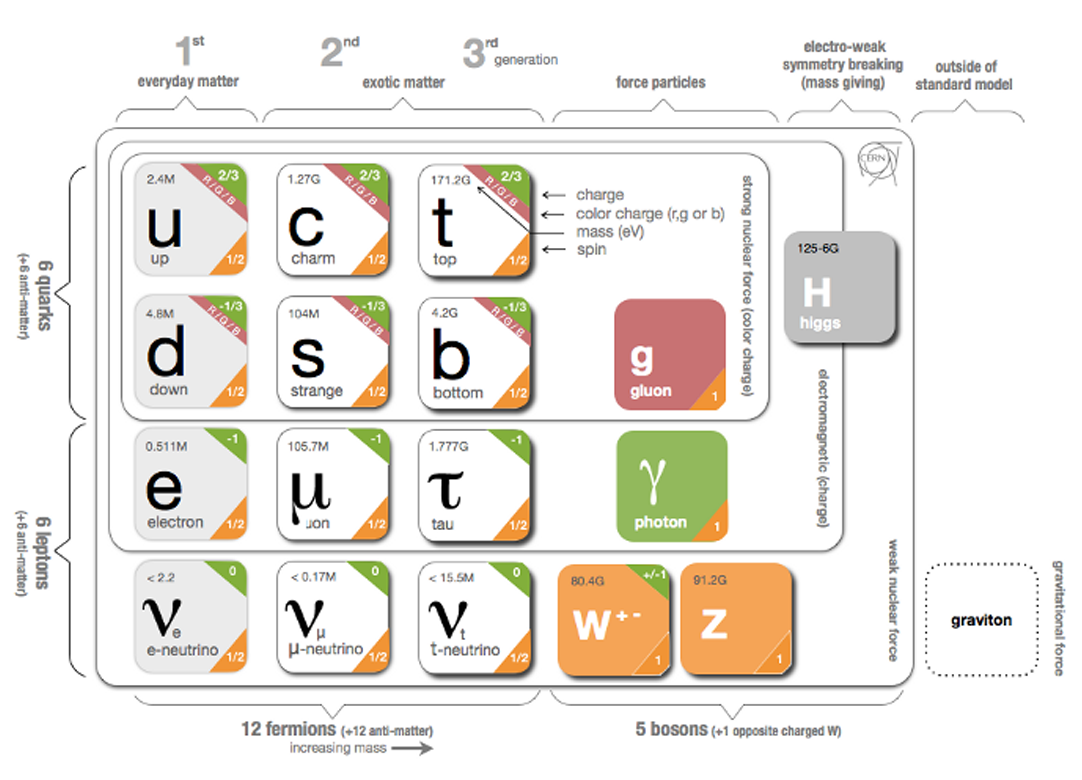
\includegraphics[width=.85\linewidth]{figures/theory/standardmodel.png}
\caption{The Standard Model of particle physics, containing all known bosons and fermions, with the addition of the hypothetical graviton. \cite{Galbraith:2012}}
\label{fig:sm}
\end{figure}
\end{centering}

\subsection{Matter}
\label{sec:matter}

The matter described by the \ac{SM} is made up of fermions, spin-$\frac{1}{2}$ particles which can be broken into two groups, quarks and leptons. The leptons all interact weakly, while the quarks additionally interact strongly. Half the leptons as well as all quarks are electromagnetically charged. 

\subsubsection{Leptons}

Leptons, as seen in the bottom left of \autoref{fig:sm}, exist in three generations, each labeled by a flavor: electron, muon, and tau. In the case of the massive leptons, these flavors are mass eigenstates, and the generations are placed in an order based on increasing mass. Each massive lepton is negatively electromagnetically charged and has a positively charged anti-particle. 

The three neutrinos exist in the same flavors as the massive leptons, but these flavor eigenstates do not correspond exactly to mass eigenstates \cite{Griffiths:111880}. As a consequence, neutrinos oscillate between flavors as they propagate through space. These oscillations are the only evidence of neutrino mass, which is bound from below by the mass splittings determined from the oscillation and bound from above my cosmological limits on the universe's mass density \cite{1979PhLB...87..144H}. Though it is still uncertain if the masses of the neutrinos follow the same hierarchy as the massive leptons, that expected ordering is slightly experimentally preferred over the inverted hierarchy \cite{Huang:2016}. 

Unlike the massive leptons, the neutrinos are not electrically charged, and it is not yet known whether each neutrino has a separate anti-particle, or if it is its own antiparticle. Because they are not electromagnetically charged, they can only interact weakly, making them extremely difficult to detect. As a consequence of their ability to evade detection, neutrinos' properties are nearly impossible to study with general purpose particle detectors. 

The \ac{SM} conserves lepton number, $L$, which is defined as the number of leptons minus the number of anti-leptons in a state, and can also be defined for each lepton flavor. Though there are anomalies that appear in second order \ac{SM} interactions which could provide very small violations of this conservation, it holds to great precision in experiment. $\mu \rightarrow e\gamma$ branching ratios, for example, have been constrained to $10^{-13}$ \cite{1605.05081}. As a consequence of this conservation, the lightest massive lepton, the electron, is stable.

\subsubsection{Quarks}
\label{sec:quarks}

Quarks, as seen in the top left of \autoref{fig:sm}, are also electromagnetically charged particles that interact weakly, but are differentiated from the leptons by their strong interactions. They are also organized in three generations ordered by mass, and come in pairs of $up$-type and $down$-type quarks, named after the lightest generation. Though the up quark is lighter than the down, that rule is reversed in the subsequent two generations. Up-type quarks are electromagnetically charged $+\frac{2}{3}$, while the down-type quarks are charged $-\frac{1}{3}$. Quarks are also charged under the strong interaction, whose three charges are often characterized by colors: red, green, and blue. Each quark has an anti-particle with the opposite charges. 

These fractional charges and individual colors are never seen in nature because of the requirement (discussed further in \autoref{sec:strong}) that stable particle states be color-neutral. To accomplish this, quarks can create two-particle bound states called \textit{mesons} consisting of one quark and one anti-quark with the same color charge, or three-particle bound states of quarks or anti-quarks with the three different color charges, which are called \textit{baryons}. The lightest color neutral state containing only quarks, the proton ($uud$), is stable. Extremely unstable bound states consisting of higher numbers of quarks can also exist, such as the pentaquark discovered in 2015 at the \ac{LHC}. \cite{Pentaquark} Collectively, these multi-quark bound states are called \textit{hadrons}. 

Like leptons, the number of quarks in a state is conserved, up to very small anomalies. However, because quarks cannot exist in an isolated state, that conservation is described in terms of baryon number ($B$) defined similarly to lepton number. Baryons are defined with $B=1$, while anti-baryons have the quantum number $B=-1$. Mesons have $B = 0$. 

\subsection{Forces}

The fermions in the previous section interact via the electromagnetic, weak, and strong forces. In a perturbative quantum field theory, interactions via these forces are represented by mediating bosons. These force carriers interact only with particles charged with their  force's quantum numbers. The photon, for example, interacts only with electromagnetically charged particles. Gluons, mediators of the strong force, interact only with color charged particles, quarks and gluons. All fermions are weakly charged and interact with the weak force's mediators, the $W$ and $Z$ bosons. 

The formulation for each of these forces is developed by requiring that the \ac{SM} Lagrangian be locally gauge invariant \cite{Griffiths:111880}. This can be accomplished by adding gauge fields to the Lagrangian, whose behavior under gauge transformations cancels out the gauge dependence of the free Lagrangian. However, adding a mass term for these fields reintroduces gauge dependence, so this mechanism only creates forces mediated by massless gauge bosons. The addition of the Higgs field provides mass terms for the weak gauge bosons (as well as other particles) without interfering with the gauge invariance. 

The total gauged symmetry group for the \ac{SM} is $SU_C(3) \times SU_L(2) \times U_Y(1)$, where $C$ stands for color, the charge of the strong force, $L$ stands for left, because the weak force is left-handed, and $Y$ is the hypercharge quantum number, the charge of the unified electroweak force. 

%\begin{equation}
%\mathcal{L}_{SM} = \mathcal{L}_{strong} + \mathcal{L}_{electroweak}
%\end{equation}

%each of which will be described in detail in their respective sections. 

\subsubsection{The Electromagnetic Force}
\label{sec:em}

Electromagnetism provides the simplest example of a requirement of local gauge invariance generating a Lagrangian description of a force.
Electromagnetism has one massless mediator, the photon, which interacts with all electromagnetically charged particles. What follows is a brief description of how enforcing this invariance generates a Lagrangian of the same form as the classical electromagnetic Lagrangian, which can be easily incorporated into the \ac{SM}. 

The particles in ~\autoref{sec:matter} are fermions, and so the Lagrangian describing their free propagation are Dirac Lagrangians and all follow the form

\begin{equation}
\mathcal{L} = i\bar{\psi}\gamma^\mu \partial_\mu\psi - m \bar{\psi}\psi . 
\end{equation}

Requiring that the free Lagrangians for these particles be invariant under a $U(1)$ local gauge transformation, $e^{iq\lambda(x)}$, can be accomplished by adding a term to the Lagrangian which cancels the derivative term arising from $\lambda$'s dependence on $x$: 

\begin{equation}
\mathcal{L} = i\bar{\psi}\gamma^\mu \partial_\mu\psi - m \bar{\psi}\psi - (q\bar{\psi}\gamma^\mu\psi)A_\mu
\end{equation}

where $A_\mu$ is a ``gauge field'' that transforms according to 

\begin{equation}
A_\mu \rightarrow A_\mu + \partial_\mu \lambda . 
\end{equation}

This vector field must also come with a free term, 

\begin{equation}
\mathcal{L} = -\frac{1}{16\pi}F^{\mu\nu}F_{\mu\nu} + \frac{1}{8\pi}m_A^2A^\nu A_\nu . 
\end{equation}

The mass term for this field would not itself be invariant under the transformation, but the field can simply be made massless to avoid this problem. The final Lagrangian, then, is 

\begin{equation}
\mathcal{L} = i\bar{\psi}\gamma^\mu \partial_\mu\psi - m \bar{\psi}\psi -\frac{1}{16\pi}F^{\mu\nu}F_{\mu\nu} - (q\bar{\psi}\gamma^\mu\psi)A_\mu
\label{eq:l_em}
\end{equation}

which is precisely the original Lagrangian with the addition of terms replicating the form of the Maxwell Lagrangian. In a quantized interpretation, it describes a field that interacts with particles with non-zero electromagnetic charge $q$ via interactions with a massless spin-1 boson, the photon. In the quantum formulization, this charge is dependent on the energy scale of the interaction, and the strength of the interaction is more typically described by the electromagnetic coupling constant

\begin{equation}
\alpha_{EM}(\mu) =  q(\mu)^2 / 4\pi . 
\end{equation}

For the purpose of succinct notation, this Lagrangian is often rewritten in terms of the \textit{covariant derivative}

\begin{equation}
D_\mu = \partial_\mu + iq\lambda A_\mu
\end{equation}

which immediately cancels the gauge dependent term created by the transformation. This mechanism is mathematically simple in the $U(1)$ case, but can be replicated for more complicated gauge transformations with perturbative approximations. 

%-------------------------------------------------------------------------------------------------------

\subsubsection{The Strong Force}
\label{sec:strong}

The strong force is generated by a similar process of requiring local gauge invariance, but in this case, for a $SU(3)$ transformation. The interactions of the strong force are described by the theory of quantum chromodynamics, which is given by the Lagrangian

\begin{equation}
\mathcal{L}_{strong} = -\frac{1}{4}G^\alpha_{\mu\nu}G^{\alpha\mu\nu} - \frac{1}{2}\bar{Q}_m \slashed{D} Q_m
\end{equation}

where the $\alpha$ index runs from 1 to 8 and represents the eight force carriers of the strong force, the gluons. $m$ indexes the three quark generations, and $G^\alpha_{\mu\nu}$ is the field strength tensor, defined as

\begin{equation}
G^\alpha_{\mu\nu} = \partial_\mu G^\alpha_\nu - \partial_\nu G^\alpha_\mu + g_s f^\alpha_{\beta\gamma}G^\beta_\mu G^\gamma_\nu
\end{equation}

where $g_s$ is a function of the energy scale of the interaction $\mu$, and is related to the strong coupling constant by

\begin{equation}
\alpha_s(\mu) =  g_s(\mu)^2 / 4\pi . 
\end{equation}

The first term of the Lagrangian gives the gluon self-coupling interactions, with terms involving 2, 3, and 4 gluon field terms. The 2-field portion is simply the field strength tensor, but the other terms give gluon self-interaction terms that can be described by the Feynman diagrams in \autoref{fig:feynman_gluons}. Unlike photons, gluons are charged by the force they carry, making self-interaction possible. 

\begin{centering}
\begin{figure}[!hbt]
\myfloatalign
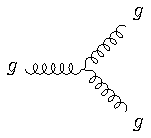
\includegraphics[width=.45\linewidth]{feynman/gluon_3.pdf}
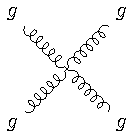
\includegraphics[width=.4\linewidth]{feynman/gluon_4.pdf}
\caption{Gluon self coupling Feynman diagrams involving 3- and 4-gluon interactions.}
\label{fig:feynman_gluons}
\end{figure}
\end{centering}

In the second term, $\slashed{D} Q_m$ is the covariant derivative acting on the quark field. The quarks are in fact charged under all three forces, strong, electromagnetic, and weak, so the covariant derivative includes terms to make each of the force's Lagrangians gauge invariant. Thus this term introduces quark-boson interactions of four types, seen in \autoref{fig:feynman_quarks}. The quarks' coupling to the gluon is the strongest, with the other couplings happening at lower rates. The couplings to the $W$ and $Z$ bosons are described in \autoref{sec:ew}.

\begin{centering}
\begin{figure}[!hbt]
\myfloatalign
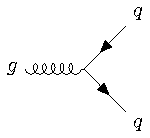
\includegraphics[width=.45\linewidth]{feynman/quark_strong.pdf}
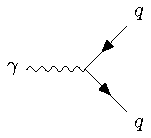
\includegraphics[width=.45\linewidth]{feynman/quark_em.pdf}
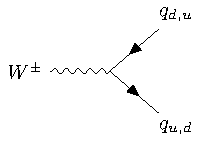
\includegraphics[width=.45\linewidth]{feynman/quark_w.pdf}
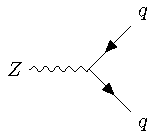
\includegraphics[width=.45\linewidth]{feynman/quark_z.pdf}
\caption{Quark couplings to the different types of gauge bosons. The $q_{u,d}$ labels represent any up- or down-type quarks.}
\label{fig:feynman_quarks}
\end{figure}
\end{centering}

%The canceling required to make the Lagrangian gauge invariant is only satisfied to a first order expansion of the transformation, guaranteeing its validity only for infinitesimally small perturbations from the ground state. 

Quantum Field Theory assumes that particles are essentially \textit{free}, propagating without interaction, and considers all interactions as purturbations on a free theory. So long as multiple interactions are much less likely than a single interaction, or put another way, so long as the coupling constants for each force are much less than one, this perturbative approximation is essentially correct. However, the strong coupling constant, $\alpha_s$, this assumption is not always valid. $\alpha_s$ changes as a function of the energy of an interaction according to its renormalization group equation

\begin{equation}
\mu^2_R \frac{d\alpha_s}{d\mu^2_R} = \beta(\alpha_s) = -(b_0\alpha_s^2 + b_1\alpha_s^3 + b_2\alpha_s^4 + ... )
\end{equation}

where $\mu^2_R$ gives the renormalization scale, and each $b_n$ gives a correction to the $\beta$-function based on diagrams with $n$ loops \cite{Agashe:2014kda}. The overall negative sign produces the unique energy dependence of $\alpha_s$, which becomes very small at high energy scales and asymptotically increases at low energies. \autoref{fig:alpha} shows this effect translated to distance scales, demonstrating that $\alpha_s<<1$ and can be considered perturbatively at small distance scales, but at large distance scales $\alpha_s$ approaches 1, and a perturbative approximation can no longer be used. Instead, for distances larger than $10^{-16}$, the colorless hadrons introduced in ~\autoref{sec:quarks} must be used to describe strong interactions.

\begin{centering}
\begin{figure}[!htb]
\myfloatalign
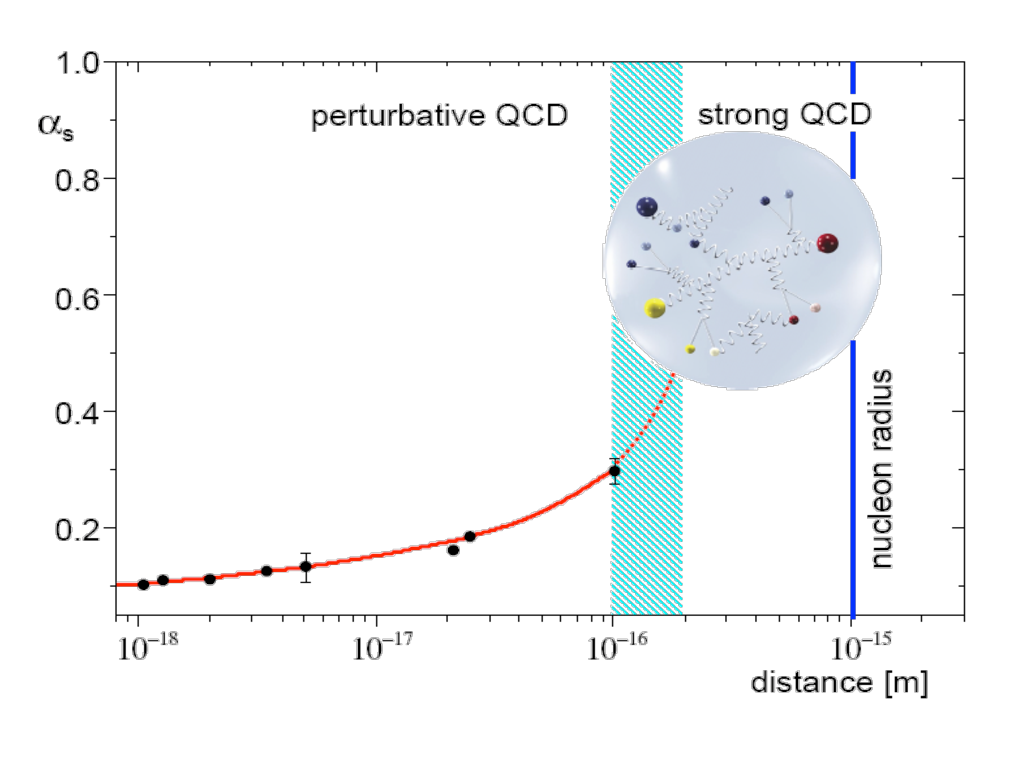
\includegraphics[width=.85\linewidth]{figures/theory/strong_coupling.png}
\caption{The running of the strong coupling constant, $\alpha_s$. \cite{Messchendorp:2013ysj}}
\label{fig:alpha}
\end{figure}
\end{centering}

The boundary between these regimes is referred to as $\Lambda_{QCD}$ and differentiates energies at which \ac{QCD} can be considered purbatively and those at which it cannot. The \ac{LHC} is capable of producing individual high-energy quarks in its hard scatterings, but they lose energy as they radiate gluons, eventually entering the energy regime below $\Lambda_{QCD}$. The transition between these two regimes is complex, and dictates the way that strongly charged particles appear in the ATLAS detector. This is described in more detail in \autoref{sec:pp_collisions}.

% \subsubsection{Quantum Chromodynamics}
% \label{sec:strong}

% \ac{QCD}, the theory describing the strong force, can be formulated similarly to the electromagnetic force, but with a $SU(3)$ transformation replacing $U(1)$. This transformation acts on a vector of equal mass quarks, the three different colors of a given flavor. The transformation is written as follows,

% \begin{equation}
% \bm{\psi} \rightarrow e^{-iq\bm{\lambda}\cdot\bm{\phi}(x)}\bm{\psi}
% \end{equation}

% where $\bm{\phi}$ gives a vector of coefficients to be multiplied by the Gell-Man matrices, $\bm{\lambda}$. Though the math is more complicated than the $U(1)$ case in this higher dimensional rotation, the cancellation is ultimately similar. 

% The main difference, corresponding to this more complicated basis of transformations, is that eight fields $A_\mu$ are required rather than the one needed in electromagnetism. These eight fields correspond to eight massless bosons, the different color states of the gluon, the carrier of the strong force.  

% All together, the total Lagrangian for \ac{QCD} is

% \begin{equation}
% \mathcal{L} = i\bar{\psi}\gamma^\mu \partial_\mu\psi - m \bar{\psi}\psi -\frac{1}{16\pi}\bm{F}^{\mu\nu}\bm{F}_{\mu\nu} - (q\bar{\psi}\gamma^\mu\psi)\bm{A}_\mu , 
% \end{equation}

% an equation identical in form to \autoref{eq:l_em}, with the mathematical complications of the additional fields hidden by the vector notation. In addition to that change, the covariant derivative must accommodate a vector $\bm{A}$ as well, changing only slightly to be defined as

% \begin{equation}
% \mathcal{D}_\mu = \partial_\mu + iq\bm{\lambda} \cdot \bm{A}_\mu .
% \end{equation}


\subsubsection{The Electroweak Force}
\label{sec:ew}

A similar process, using an $SU(2)$ gauge transformation, can produce a Lagrangian that would suffice to describe the $W$ and $Z$ bosons of the \ac{SM}, if only they were massless. However, they are not, so an alternate mechanism is needed to generate massive force carriers. 

Before a mechanism for their masses was understood, and before they were discovered, the large masses of the $W$ and $Z$ bosons were proposed in order to unify the electromagnetic and weak forces into the electroweak force \cite{Griffiths:111880}. The large masses were crucial to explain the discrepancy in the strength of the two forces. 

The unified electroweak force is generated by a symmetry group written as ${SU(2)_L \times U(1)_Y}$, where $L$ refers to left-handed fields, and $Y$ is the quantum number for \textit{hypercharge}. This new quantum number is defined as 

\begin{equation}
Y = 2(Q - T_3)
\end{equation}

where $Q$ is the electromagnetic charge and $T_3$ is the third component of weak isospin $\bm{T}$, the quantum number relating to the weak interaction. In the unified theory, quark and lepton singlets interact according to their hypercharge, and left-handed quarks and leptons, grouped according to their generation, interact as doublets. 

The gauge bosons resulting from this unified theory include a triplet, $\bm{W}$, with coupling $g_W$, and a singlet field $B$, with coupling $g'/2$. However, the electroweak symmetry is broken, and mixing between these states occurs. Rewritten in their mass basis, the standard electroweak force carriers are produced: $W^\pm$, two states with identical coupling resulting from the first two states of the $\bm{W}$ triplet, the $Z$ and the photon field $A$ resulting from the mixing of the last $\bm{W}$ state and $B$. 

The electroweak Lagrangian is much more complicated than the strong Lagrangian, and can be divided into several terms:

\begin{equation}
\mathcal{L}_{electroweak} = \mathcal{L}_{gauge} + \mathcal{L}_{fermions} + \mathcal{L}_{Higgs} + \mathcal{L}_{Yukawa} .
\end{equation}

The first term can be written as follows

\begin{equation}
\mathcal{L}_{gauge} = -\frac{1}{4}W^{a\mu\nu}W^a_{\mu\nu} - \frac{1}{4}B^{\mu\nu}B{\mu\nu} 
\end{equation}

where the $a$ indices are numbered 1 through 3 and indicate the generators of $SU(2)$ which are written 

\begin{equation}
W^a_{\mu\nu} = \partial_\mu W^a_\nu - \partial_\nu W^a_\mu + g_2 \epsilon_{abc} W^b_\mu W^c_\nu
\end{equation}

The gauge portion of the Lagrangian then generates interaction terms of between the gauge fields, which when rewritten in terms of the mass-eigenstate basis, generates interactions between three gauge bosons, like the ones in \autoref{fig:tlgc}, as well as interactions between four gauge bosons.

\begin{centering}
\begin{figure}[!hbt]
\myfloatalign
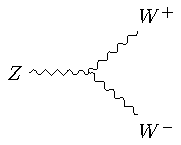
\includegraphics[width=.45\linewidth]{feynman/tlgc_z.pdf}
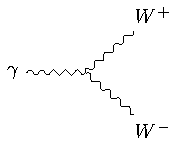
\includegraphics[width=.45\linewidth]{feynman/tlgc_g.pdf}
\caption{Feynman diagrams of trilinear gauge couplings in the \ac{SM}.}
\label{fig:tlgc}
\end{figure}
\end{centering}

The fermion portion of the Lagrangian is written as

\begin{equation}
\begin{split}
\mathcal{L}_{fermion} = & -\frac{1}{2}\bar{L}_m\slashed{D}L_m -\frac{1}{2}\bar{Q}_m\slashed{D}Q_m \\
						& -\frac{1}{2}\bar{U}_m\slashed{D}U_m -\frac{1}{2}\bar{D}_m\slashed{D}D_m \\
						& -\frac{1}{2}\bar{E}_m\slashed{D}E_m \\
\end{split}
\end{equation}

where $L$ is the left-handed lepton doublet, $Q$ is the left-handed quark doublet, $U$ is the right-handed singlet for up-type quarks, $D$ is the same for down-type quarks, and $E$ is the right-handed singlet for electrons, muons and taus. Each of these fields has an implicit index running from 1 to 3 to represent the three generations. The covariant derivative in each term includes terms including all the gauge fields the fermion is charged under. Unlike the other forces, the weak force treats left- and right-handed fermion fields differently; it only interacts with the left-handed fields, so only the first two terms' covariant derivatives include $\bm{W}$ terms. The first term in this Lagrangian, for example, produces weak interactions depicted in \autoref{fig:feynman_weak}. The $Z$ bosons, because they represent a mixing between the $\bm{W}$ and $B$ fields, can interact with right-handed leptons and quarks, but do so with different strengths than left-handed particles.

\begin{centering}
\begin{figure}[!hbt]
\myfloatalign
\includegraphics[width=.45\linewidth]{feynman/weak_wplus.pdf}
\includegraphics[width=.45\linewidth]{feynman/weak_wminus.pdf}
\includegraphics[width=.45\linewidth]{feynman/weak_zll.pdf}
\includegraphics[width=.45\linewidth]{feynman/weak_zvv.pdf}
\caption{Feynman diagrams of weak couplings to leptons in the \ac{SM}.}
\label{fig:feynman_weak}
\end{figure}
\end{centering}

No right-handed term appears for the neutrino field, because only left-handed neutrinos and right-handed anti-neutrinos have been observed. However, because neutrinos have non-zero mass, their chirality can change with frame boosts, which complicates any claim that right-handed neutrinos do not exist \cite{Burgess:2007zi}. It is possible that neutrinos are their own antiparticle, making the right-handed anti-neutrino the solution to this problem. It's also possible that very massive right-handed neutrinos do exist, and simply haven't been discovered yet. 

The remaining two terms of the electroweak Lagrangian are related to the Higgs field, which is the source of electroweak symmetry breaking. 

\subsubsection{The Higgs Mechanism}

The Higgs mechanism presents a way to generate a mass term for the electroweak gauge bosons. It is a scalar field, with a Lagrangian 

\begin{equation}
\mathcal{L}_{Higgs} = \frac{1}{2}(\partial_\mu\phi)^*(\partial^\mu\phi) + \frac{1}{2}\mu^2\phi^*\phi - \frac{1}{4}\lambda^4(\phi^*\phi)^2
\end{equation}

where $\phi$ is a complex scalar field, $\phi = \phi_1 + i\phi_2$. This looks very similar to a standard scalar field Lagrangian, but the signs on the mass and interaction terms are reversed, implying an imaginary mass term. However, this isn't a good interpretation of the Lagrangian, because it differs from all previously considered Lagrangians in one important way: its ground state does not occur at $\phi = 0$. Because quantum field theory is perturbative, its validity only holds when expanded around a ground state, which, when calculated for this Higgs Lagrangian, must satisfy

\begin{equation}
\phi_1^2 + \phi_2^2 = \frac{\mu^2}{\lambda^4} . 
\end{equation}

The original Lagrangian can then be rewritten in terms of a field $v + H(x)$ centered around the ground state with energy called the vacuum expectation value defined as. 

\begin{equation}
v = \frac{\mu}{\lambda^2} . 
\end{equation}

This rewriting produces a Lagrangian with a non-imaginary mass. However, in an effect called \textit{spontaneous symmetry breaking}, the original $SO(2)$ rotational symmetry of the Lagrangian is lost, resulting only in a $U(1)$ rotational symmetry; the Lagrangian is invariant under a phase transformation.

As in \autoref{sec:em}, it is possible to make the Lagrangian invariant under a local $U(1)$ transformation, $\phi \rightarrow e^{i\theta(x)\phi}$ by adding a massless gauge field $A^\mu$ and using the covariant derivative. Due to the many cross terms from the non-zero ground state, terms for the mass of one of the scalar bosons as well as the gauge field appear, leaving only one massless scalar boson. This massless boson, it turns out, can be completely removed from the theory via local $U(1)$ transformations, ultimately producing a theory with one massive scalar (the Higgs) and a massive gauge field ($\bm{W}$). 

The Higgs interaction with the weak gauge bosons also creates couplings between the particles, which can be seen in \autoref{fig:higgs_gauge}. There are also Higgs self-interation terms included in the Lagrangian, producing vertices describing 3- and 4-Higgs interactions. 

\begin{centering}
\begin{figure}[!hbt]
\myfloatalign
\includegraphics[width=.45\linewidth]{feynman/higgs_ww.pdf}
\includegraphics[width=.41\linewidth]{feynman/higgs_zz.pdf}
\includegraphics[width=.45\linewidth]{feynman/higgs_hhww.pdf}
\includegraphics[width=.40\linewidth]{feynman/higgs_hhzz.pdf}
\caption{Feynman diagrams demonstrating Higgs couplings to the weak gauge bosons in the \ac{SM}.}
\label{fig:higgs_gauge}
\end{figure}
\end{centering}

The remaining piece of the Lagrangian, $\mathcal{L}_{Yukawa}$ describes the Higgs field's interactions with the fermions of the \ac{SM}, and can be written as

\begin{equation}
\mathcal{L}_{Yukawa} = -\Gamma^e_{mn}\bar{L}_m \phi E_n -\Gamma^u_{mn}\bar{Q}_m \phi U_n -\Gamma^d_{mn}\bar{Q}_m \phi D_n + h.c.
\end{equation} 

where $h.c.$ is the hermitian conjugate term, and the $\Gamma$ matrices are indexed by generation, and, when diagonalized, are proportional to the masses of the fermions. The Higgs field's vacuum expectation value produces terms that look like fermion mass terms. Additionally, terms that couple the fermions to the Higgs field are produced, with each fermion's coupling proportional to its mass, according to 

\begin{equation}
\mathcal{g}_{f} = \sqrt{2}\frac{m_f}{v}
\end{equation}

where $m_f$ is the mass of the fermion. Feynman diagrams for lepton and quark terms can be seen in \autoref{fig:higgs_fermion}.

 \begin{centering}
\begin{figure}[!hbt]
\myfloatalign
\includegraphics[width=.45\linewidth]{feynman/higgs_ll.pdf}
\includegraphics[width=.45\linewidth]{feynman/higgs_qq.pdf}
\caption{Feynman diagrams showing Higgs couplings to fermions in the \ac{SM}.}
\label{fig:higgs_fermion}
\end{figure}
\end{centering}

% The original Lagrangian can be put in terms of $\eta$ and $\xsi$, defined as

% \begin{equation}
% \eta = \phi_1 \pm \frac{\mu}{\lambda}  ; \xsi = \phi_2
% \end{equation}

% to read

% \begin{equation}
% \mathcal{L} = \frac{1}{2}(\partial_\mu\eta)(\partial^\mu\eta) - \mu^2\eta^2 \pm \mu\lambda\eta^3 - \frac{1}{4}\lambda^2\eta^4 + \frac{1}{4}(\frac{\mu^2}{\lambda})^2 . 
% \end{equation}

% This Lagrangian now has a reasonable mass term ($m = \sqrt{2}\mu$) and several interaction terms. However, it no longer shares a symmetry of the original Lagrangian; though $\mathcal{L}$ is invariant under $\phi \rightarrow e^{i\theta}\phi$, it is not invariant under $\eta \rightarrow e^{i\theta}\eta$. This is referred to as spontaneous symmetry breaking. 

\subsection{Phenomenology of Proton-Proton Collisions}
\label{sec:pp_collisions}

As discussed in \autoref{ch:lhc}, the \ac{LHC} collides bunches of high-energy protons, and the interactions of these protons' constituent quarks produce the wide array of particles seen in the ATLAS detector. The \ac{LHC} typically cites its energy in terms of $\sqrt{S}$, the center of mass energy of protons in the two colliding beams, which in Run 2 is 13\tev. However, because the proton is not fundamental, this energy is divided among many particles that make up the proton. 

To first order, a proton consists of three quarks: two up quarks and one down quark. However, a real quantum mechanical system is much more chaotic, with other quarks popping into and out of existence and gluons flying between them. These additional quarks are called \textit{sea} quarks and can also carry fractions of the proton's energy.

The particles inside the proton can have a wide range of energies depending on the internal dynamics at the moment of the collision. These cannot be predicted exactly, but probabalistic models called \acfp{PDF} describe the likelihood of any given configuration. These models are determined using data from hard scattering experiments and give probabalistic estimates for how often a given type of particle appears with a fraction $x$ of the total proton energy, as seen in \autoref{fig:pdf}. 

\begin{centering}
\begin{figure}[bth]
\myfloatalign
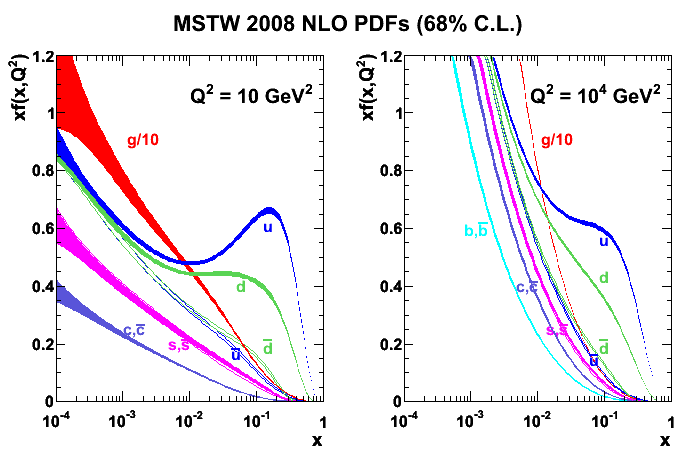
\includegraphics[width=.85\linewidth]{figures/theory/mstw2008nlo68cl_allpdfs.png}
\caption{2008 MSTW \acp{PDF} for various particle types given as a function of $x$ and $Q^2$, the square of the parton-parton momentum transfer. \cite{0901.0002}}
\label{fig:pdf}
\end{figure}
\end{centering}



%------------------------------------------------

\subsection{Problems in the Standard Model}
\label{sec:sm_problems}

Thought the \ac{SM} is a self-consistent theory that describes to great accuracy all of the particles and forces it includes, it does have certain shortcomings. The most glaring is the omission of gravity. Though the force is well understood at large scales via the theory of General Relativity, no satisfying quantum description of gravity has been accepted, much less proven. The Planck scale, the energy scale at which gravitational interactions become large enough that no sound theory can ignore gravity, is at about $10^{28}$ \eV, 16 orders of magnitude above the electroweak scale, so the exclusion of gravity from the \ac{SM} is unlikely to directly affec \ac{LHC} physics. 

Another clear omission of the \ac{SM} is \acf{DM}. This matter was first identified in 1933 through the observation of galactic rotation curves. \cite{zwicky} The speed of rotation indicated both that there was more mass in the system than could be accounted for by observations made directly of the galaxy, and that this additional matter was distributed in a halo, not a disk like the typical luminous matter. This effect can be seen in \autoref{fig:dm_curve}. Since then, the gravitational impact of \ac{DM} has been observed in colliding clusters and many more rotational curves, but the particles that form \ac{DM} have never been directly detected or seen at a particle accelerator. As a consequence, very few details are known about the nature of this matter, only its density throughout the universe and that it does not interact strongly or electromagnetically. 

\begin{centering}
\begin{figure}[bth]
\myfloatalign
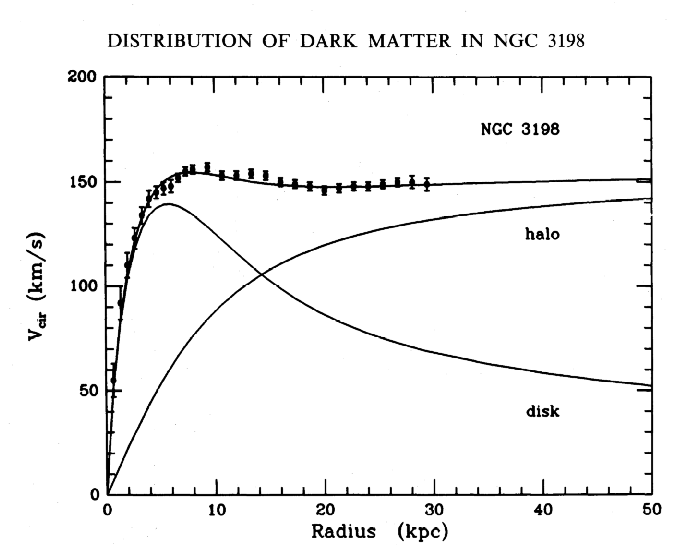
\includegraphics[width=.85\linewidth]{figures/theory/rotatioanl_curve_ngc3198_rc.png}
\caption{Galactic rotation curve showing that the discrepancy between the observed luminous matter and the total mass in the system can be described as a non-luminous halo of matter. \cite{1985ApJ...295..305V}}
\label{fig:dm_curve}
\end{figure}
\end{centering}

Beyond the omissions of the \ac{SM}, there are several aesthetic problems - ones that could have no solution, but seem to suggest that the current \ac{SM} are missing some pieces that could unify it and provide more order. The first is the sheer number of parameters in the \ac{SM}. There are 26 independent parameters determining the mass of the particles and all the couplings between them. Besides the rough grouping of fermions into generations, there seems to be no order to masses of particles, and no way to predict the masses or couplings. Each, it seems, is independently provided by nature. 

In the past, large numbers of seemingly unrelated parameters have indicated that a theory has a more fundamental form at shorter distance scales. The large number of elements, it turned out, could be explained by different groupings of three particles, the proton, neutron and electron. Later, the menagerie of hadrons became so large that a similar reimagining of what was fundamental took place, and the theory of quarks gave an order to the many mesons and baryons. This pattern leaves physicists suspicious of any theory with too many particles and free parameters, suggesting that perhaps, at a higher energy, there is a simpler model that can unify many of the seemingly disparate elements of the \ac{SM}. 

In addition, some of these seemingly independent parameters have suspicious symmetry. The Higgs mass, for example, has been measured to be 125 \gev. This mass is the sum of the bare mass, the one that appears in the Lagrangian, and quantum corrections from interactions with other particles, which are proportional to the square of the particles' mass. Since new physics must exist at the Planck scale to account for gravity, these corrections could be up to 35 orders of magnitude larger than the Higgs mass. Though the bare mass could theoretically cancel out this massive correction, these parameters should be independent, and the odds that they would be precisely the same to 35 places are very, very small. This near-exact canceling is often called \textit{fine-tuning}, an undesirable trait in a theory which suggests that some more fundamental symmetry has been missed. A \textit{natural} solution, one free of this fine-tuning, is sought to resolve this \ac{SM} problem. 

%-------------------------------------------------

\section{Supersymmetry}

\acf{SUSY} was proposed and developed in the 1970s to give solutions to many of these \ac{SM} shortcomings. The theory works by introducing a fermionic symmetry to the \ac{SM}, in addition to the usual spacetime symmetries of translations, rotations, and changes of Lorentz frame. The combination of the usual spacetime with this fermionic dimension is called a \textit{superspace}. Rotations in this dimension result in a particle's spin changing by 1/2, turning a spin-1/2 fermion into a spin-0 particle, for example. As a consequence, this symmetry requires the existence of many new particles - a bosonic \textit{sfermion} for each fermion of the \ac{SM} and a fermionic \textit{gaugino} for each of the gauge bosons. These superpartners of \ac{SM} particles should have identical quantum numbers to the original particle, except for their spins. \autoref{tab:sparticles} shows the \ac{SM} particles and their superpartners. 

%TODO make better figure

\begin{table}
\begin{center}
 \begin{tabular}{cc|c|c|c}
   \hline 
   \multicolumn{2}{c|}{Names} & sparticles & particles & $SU(3)_C, SU(2)_L, U(1)_Y$ \\
   \hline
   \hline
   \multirow{3}{*}{squarks, quarks} & $Q$ 		& ($\squ[L] \sqd[L]$) & ($u_L d_L$) 		& ($\bf{3}, \bf{2}, \frac{1}{6}$) 		\\
   									& $\squ$ 	& $\squ[R]^*$ 		& $u^\dagger_R$ 	& ($\bf{\bar{3}}, \bf{1}, -\frac{2}{3}$) 	\\
   									& $\sqd$ 	& $\sqd[R]^*$ 		& $d^\dagger_R$ 	& ($\bf{\bar{3}}, \bf{1}, \frac{1}{3}$) 	\\		
   \hline
   \multirow{2}{*}{sleptons, leptons} & $L$ 	& ($\slneu \sle[L]$) & ($\nu e_L$) 		& ($\bf{1}, \bf{2}, -\frac{1}{2}$) 		\\
   									& $\bar{e}$ & $\sle[R]^*$ 		& $e^\dagger_R$ 	& ($\bf{1}, \bf{1}, 1$) 					\\
   \hline
   \multirow{2}{*}{Higgs, higgsinos} & $H_u$ 	& ($\Hou[+] \Hou[0]$) 	& ($H^+_u H^0_u$)  & ($\bf{1}, \bf{2}, \frac{1}{2}$) 	\\
   									& $H_d$ 	& ($\Hod[0] \Hod[-]$) 	& ($H^0_d H^-_d$)  & ($\bf{1}, \bf{2}, -\frac{1}{2}$) 	\\  
   \hline
   \multicolumn{2}{c|}{gluino, gluon}	& $\go$ 			& $g$			& ($\bf{8}, \bf{1}, 0$)		\\							
   \hline
   \multicolumn{2}{c|}{winos, $W$ bosons}	& $\Wo^\pm \Wo^0$ 	& $W^\pm W^0$	& ($\bf{1}, \bf{3}, 0$)		\\							
   \hline
   \multicolumn{2}{c|}{bino, $B$ boson}	& $\Bo^0$ 			& $B^0$			& ($\bf{1}, \bf{1}, 0$)		\\							

\hline
\hline
 \end{tabular}
\end{center}
 \caption{Supermultiplets of the \ac{MSSM}. Sfermions, on the first five rows, are all spin-0. Higgsinos and gauginos are all spin-1/2. Three sets of each fermion's supermultiplet exist, one for each generation. \cite{Martin:1997ns}}
 \label{tab:sparticles}
\end{table}


If the theory is symmetric under these fermionic rotations, these particle-sparticle pairs can be described by a single \textit{superfield}, which simultaneously describes the behavior of both \ac{SM} and \ac{SUSY} particles in the superspace. However, this completely symmetric behavior is untenable given basic observations of matter in the universe. For example, if there were a \textit{selectron} (the superpartner of the electron, $\sle$), with identical mass to the electron, it would have been detected long ago. In fact, such a particle would fundamentally change atomic structure, with the bosonic selectrons capable of piling into the ground state of an atom, and removing all the interesting valence-shell interactions of electrons that determine molecular structure. Thus, if \ac{SUSY} does exist, the symmetry must be broken, with much higher masses for the superpartners than the original \ac{SM} particles. 

\subsection{The Minimal Supersymmetric Standard Model}

The \acf{MSSM} was designed to be the simplest supersymmetric extension of the \ac{SM} that remains self consistent, and it results in the particles seen in \autoref{tab:sparticles}\cite{Martin:1997ns}. The formulation of the \ac{MSSM} begins by introducing a second Higgs doublet to account for the different masses of the sparticles. As with the \ac{SM} Higgs, electroweak symmetry breaking results in the loss of degrees of freedom, and only five of the original eight states remain, the lightest of which, $h^0$, can be interpreted as the \ac{SM} Higgs already discovered. There are two remaining neutral states, $A^0$ and $H^0$, as well as two charged Higgses, $H^\pm$. 

The neutral Higgs states mix with the neutral gauge bosons, while the charged Higgs states mix with the charged gauge bosons, producing a series of states labeled only by their charge and the order of their masses. The neutral states, collectively called the neutralinos, are identified from lightest to heaviest, $\No[1], \No[2], \No[3],$ and $\No[4]$. The charged states, referred to as charginos, are similarly called $\Co[1]$ and $\Co[2]$.

The \ac{MSSM} introduces many new interactions between \ac{SM} particles and sparticles. Though these don't represent all possible interactions, a general rule is that any \ac{SM} vertex can have two interacting particles replaced with their sparticle equivalents, and this vertex will be part of the \ac{MSSM}. \autoref{fig:mssm_int} gives two examples of such vertices. 

\begin{centering}
\begin{figure}[!hbt]
\myfloatalign
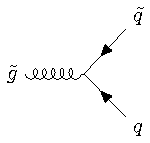
\includegraphics[width=.45\linewidth]{feynman/gluino.pdf}
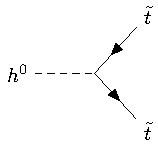
\includegraphics[width=.45\linewidth]{feynman/higgs_stop.pdf}
\caption{Two example vertices allowed by the \ac{MSSM}.}
\label{fig:mssm_int}
\end{figure}
\end{centering}

In addition to these interactions, there are several terms that appear in the \ac{MSSM} Lagrangian that violate the $B$ and $L$ conservation observed in the \ac{SM}. In fact, these terms violate $B-L$, which, unlike $B$ and $L$ conservation individually, does not have even small violations in the \ac{SM}. These superpotential terms appear as follows

\begin{eqnarray}
W_{\Delta L = 1} = \frac{1}{2}\lambda^{ijk}L_i L_j \bar{e}_k + \lambda'^{ijk}L_i Q_j \bar{d}_k + \mu'^i L_i H_u \\
W_{\Delta B = 1} = \frac{1}{2}\lambda''^{ijk}\bar{u}_i \bar{d}_j \bar{d}_k .
\label{eq:rviol}
\end{eqnarray}

Because there are very strong limits on non-conservation of $B-L$ from proton decay experiments, these terms present a challenge for the \ac{MSSM}. It would be possible, of course, to simply tune the $\lambda$ parameters to be small enough to fit within experimental constraints, but these terms can also be eliminated by introducing a new conserved quantity, $R$-parity. It is defined by

\begin{equation}
P_R = -1^{3(B-L)+2s}
\end{equation}

where $s$ is the spin of the particle. Requiring that all terms in the Lagrangian have a multiplicative $P_R$ of 1 excludes the terms in \autoref{eq:rviol}, removing the problem of proton decay. All \ac{SM} particles are $R$-parity even, while the sparticles are $R$-parity odd, so the conservation of $R$-parity can translate into a conservation of number of particles and sparticles. As a consequence, massive sparticles typically decay through a chain of lighter sparticles, emitting \ac{SM} particles along the way.  

\subsection{Solutions to Standard Model Problems}

Perhaps the most compelling consequence of \ac{SUSY} comes from $R$-parity, which, through the formation of a new quantum number unique to sparticles, requires the \acf{LSP} to be stable. This stable particle, if it is neutrally charged, provides an excellent candidate \ac{DM} particle. The lightest neutralino, for example, is a viable \ac{DM} candidate because it does not interact electromagnetically or strongly, a constraint required due to measurements of the relic density of \ac{DM} in the universe. An interaction cross-section higher than what's expected for weak interactions would have led the \ac{DM} particle and its anti-particle to annihilate at lower densities, leaving a much smaller amount of \ac{DM} in the universe than what is observed today \cite{astro-ph/9407006}.

Many believe that a complete \ac{SM} would include a unification of the three forces, as electromagnetism and the weak force have already been unified. This requires that at some higher energy, the coupling constants of all three forces merge. However, in the \ac{SM}, the coupling constants come close to aligning, but don't perfectly cross. With the addition of \ac{MSSM} particles with masses at the \tev~scale, the alignment is near perfect, as shown in \autoref{fig:gut_mssm}. This may be a mathematical coincidence, but it's very compelling to those physicists who believe that ``Grand Unified Theory'' must exist. 

\begin{centering}
\begin{figure}[!hbt]
\myfloatalign
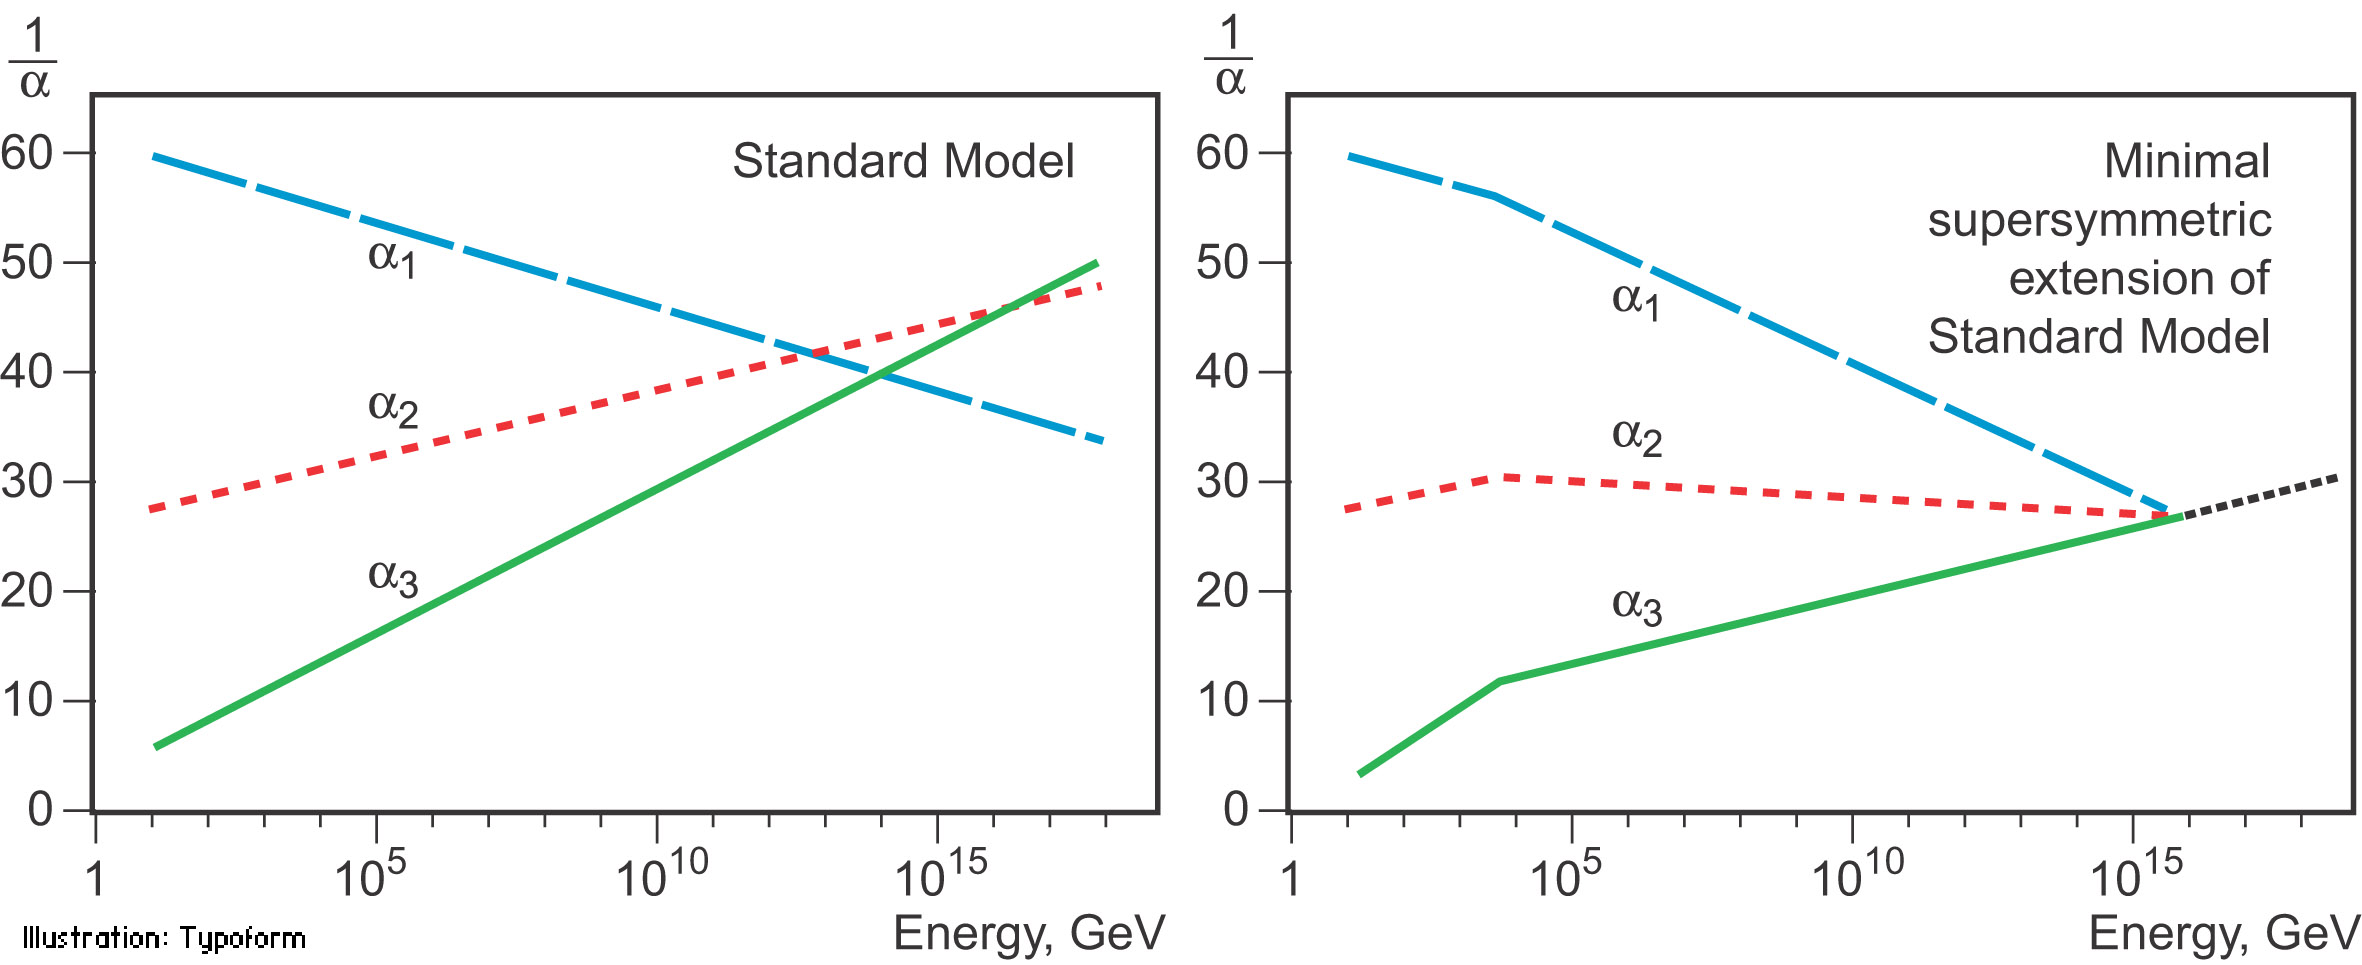
\includegraphics[width=.9\linewidth]{figures/theory/phypub4highen.jpg}
\caption{Running of the strong, weak, and electromagnetic coupling constants for the \ac{SM} (left) and \ac{MSSM} (right). \cite{nobel2004}}
\label{fig:gut_mssm}
\end{figure}
\end{centering}

\ac{SUSY} also has the potential to solve the naturalness problem in the \ac{SM}. In the \ac{SM}, the massive amounts of fine tuning are required to cancel the quadratic corrections to the Higgs mass that result from loops involving, most importantly, the top quark. In the \ac{MSSM}, an similar loop involving the stop quark (the vertex for which is depicted in \autoref{fig:mssm_int}) contributes to the Higgs mass with the opposite sign, making it possible to naturally cancel the corrections without fine tuning. However, the larger the mass difference between the top quark and stop quark, the larger the remaining correction when the two terms cancel. Consequentially, to preserve a reasonable degree of naturalness (and here the definition of ``reasonable'' is subject to some debate), the stop quark should appear at masses not too much larger than the top's, at approximately the \tev~scale. 

This naturalness mass limit, as well as the unification of couplings, make the argument for searching for \ac{SUSY} at the \ac{LHC} particularly compelling, as the \ac{LHC} is the first collider capable of producing particles at the \tev~scale. As new exclusions on \ac{SUSY} are set, the remaining phase space becomes slightly less natural, but there is no shortage of unexcluded \ac{SUSY} theories, which are continually proposed as new limits are created. 

\subsection{Simplified Models of Supersymmetry}
\label{sec:simplified_models}

There are many different theorized models of \ac{SUSY}, with different mechanisms for breaking the symmetry. Each of these theories typically contains on order hundreds of free parameters, with complex interactions that determine the mass hierarchy and interaction rates of the sparticles. From an experimental point of view, the details of these theories and the exact way the hierarchies are generated are often less relevant to a search than their outputs. 

Simplified models, which are typically inspired by more complete theories, are used to tune the observables of a model more directly. These models each consist of one production and decay diagram, with the masses of the particles free to be tuned directly. In a more complete theory, it is instead necessary to modify more fundamental parameters like the symmetry breaking scale. A change like this impacts the properties of all the sparticles, but the details of its impact are model dependent. The simplified models allow for relatively model independent interpretations that can also be reinterpreted in the context of a more complete \ac{SUSY} theory.

In the analysis presented in \autoref{part:search}, a simplified model is used which produces the decay depicted in \autoref{fig:simpmodel}. This decay chain begins with the pair production of gluinos, which decay via a pair of quarks to the second lightest neutralino, which then decay via a $Z$ boson to the lightest neutralino. In this simplified model, the lightest neutralino is the \ac{LSP}, and is stable.

\begin{centering}
\begin{figure}[!hbt]
\myfloatalign
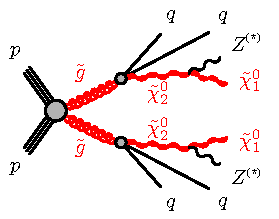
\includegraphics[width=.9\linewidth]{figures/theory/gogo-qqqqZZN1N1.pdf}
\caption{Feynman diagram of the decay considered in the simplified models used in the analysis presented in \autoref{part:search}.}
\label{fig:simpmodel}
\end{figure}
\end{centering}

Using this simplified model, the masses of the particles can be tuned directly. This is very helpful for the generation of \ac{MC}, discussed in \autoref{sec:MC_gen}, because a grid of different mass values of the important sparticles involved in the decay can be generated, allowing analyzers to make predictions of likely signals, and to exclude the simplified models as a function of the mass of the sparticles in the case that no discrepancies between predictions and observations are seen. 

\subsubsection{Context and Motivation}

Processes similar to the one described by \autoref{fig:simpmodel} have been the target of previous \ac{LHC} searches. Both \ac{CMS} and ATLAS performed searches for \ac{SUSY} in the two lepton channel with the 8 \tev~data collected in 2012. The ATLAS search saw a 3$\sigma$ excess, shown in \autoref{fig:atlas_8tev} \cite{SUSY-2014-10}. The \ac{CMS} search saw no excess in a similarly motivated signal region, albeit with different kinematic cuts than ATLAS's, following up on a 7 \tev~search that saw no excess \cite{Chatrchyan:2012qka, CMS2}. 

\begin{centering}
\begin{figure}[!hbt]
\myfloatalign
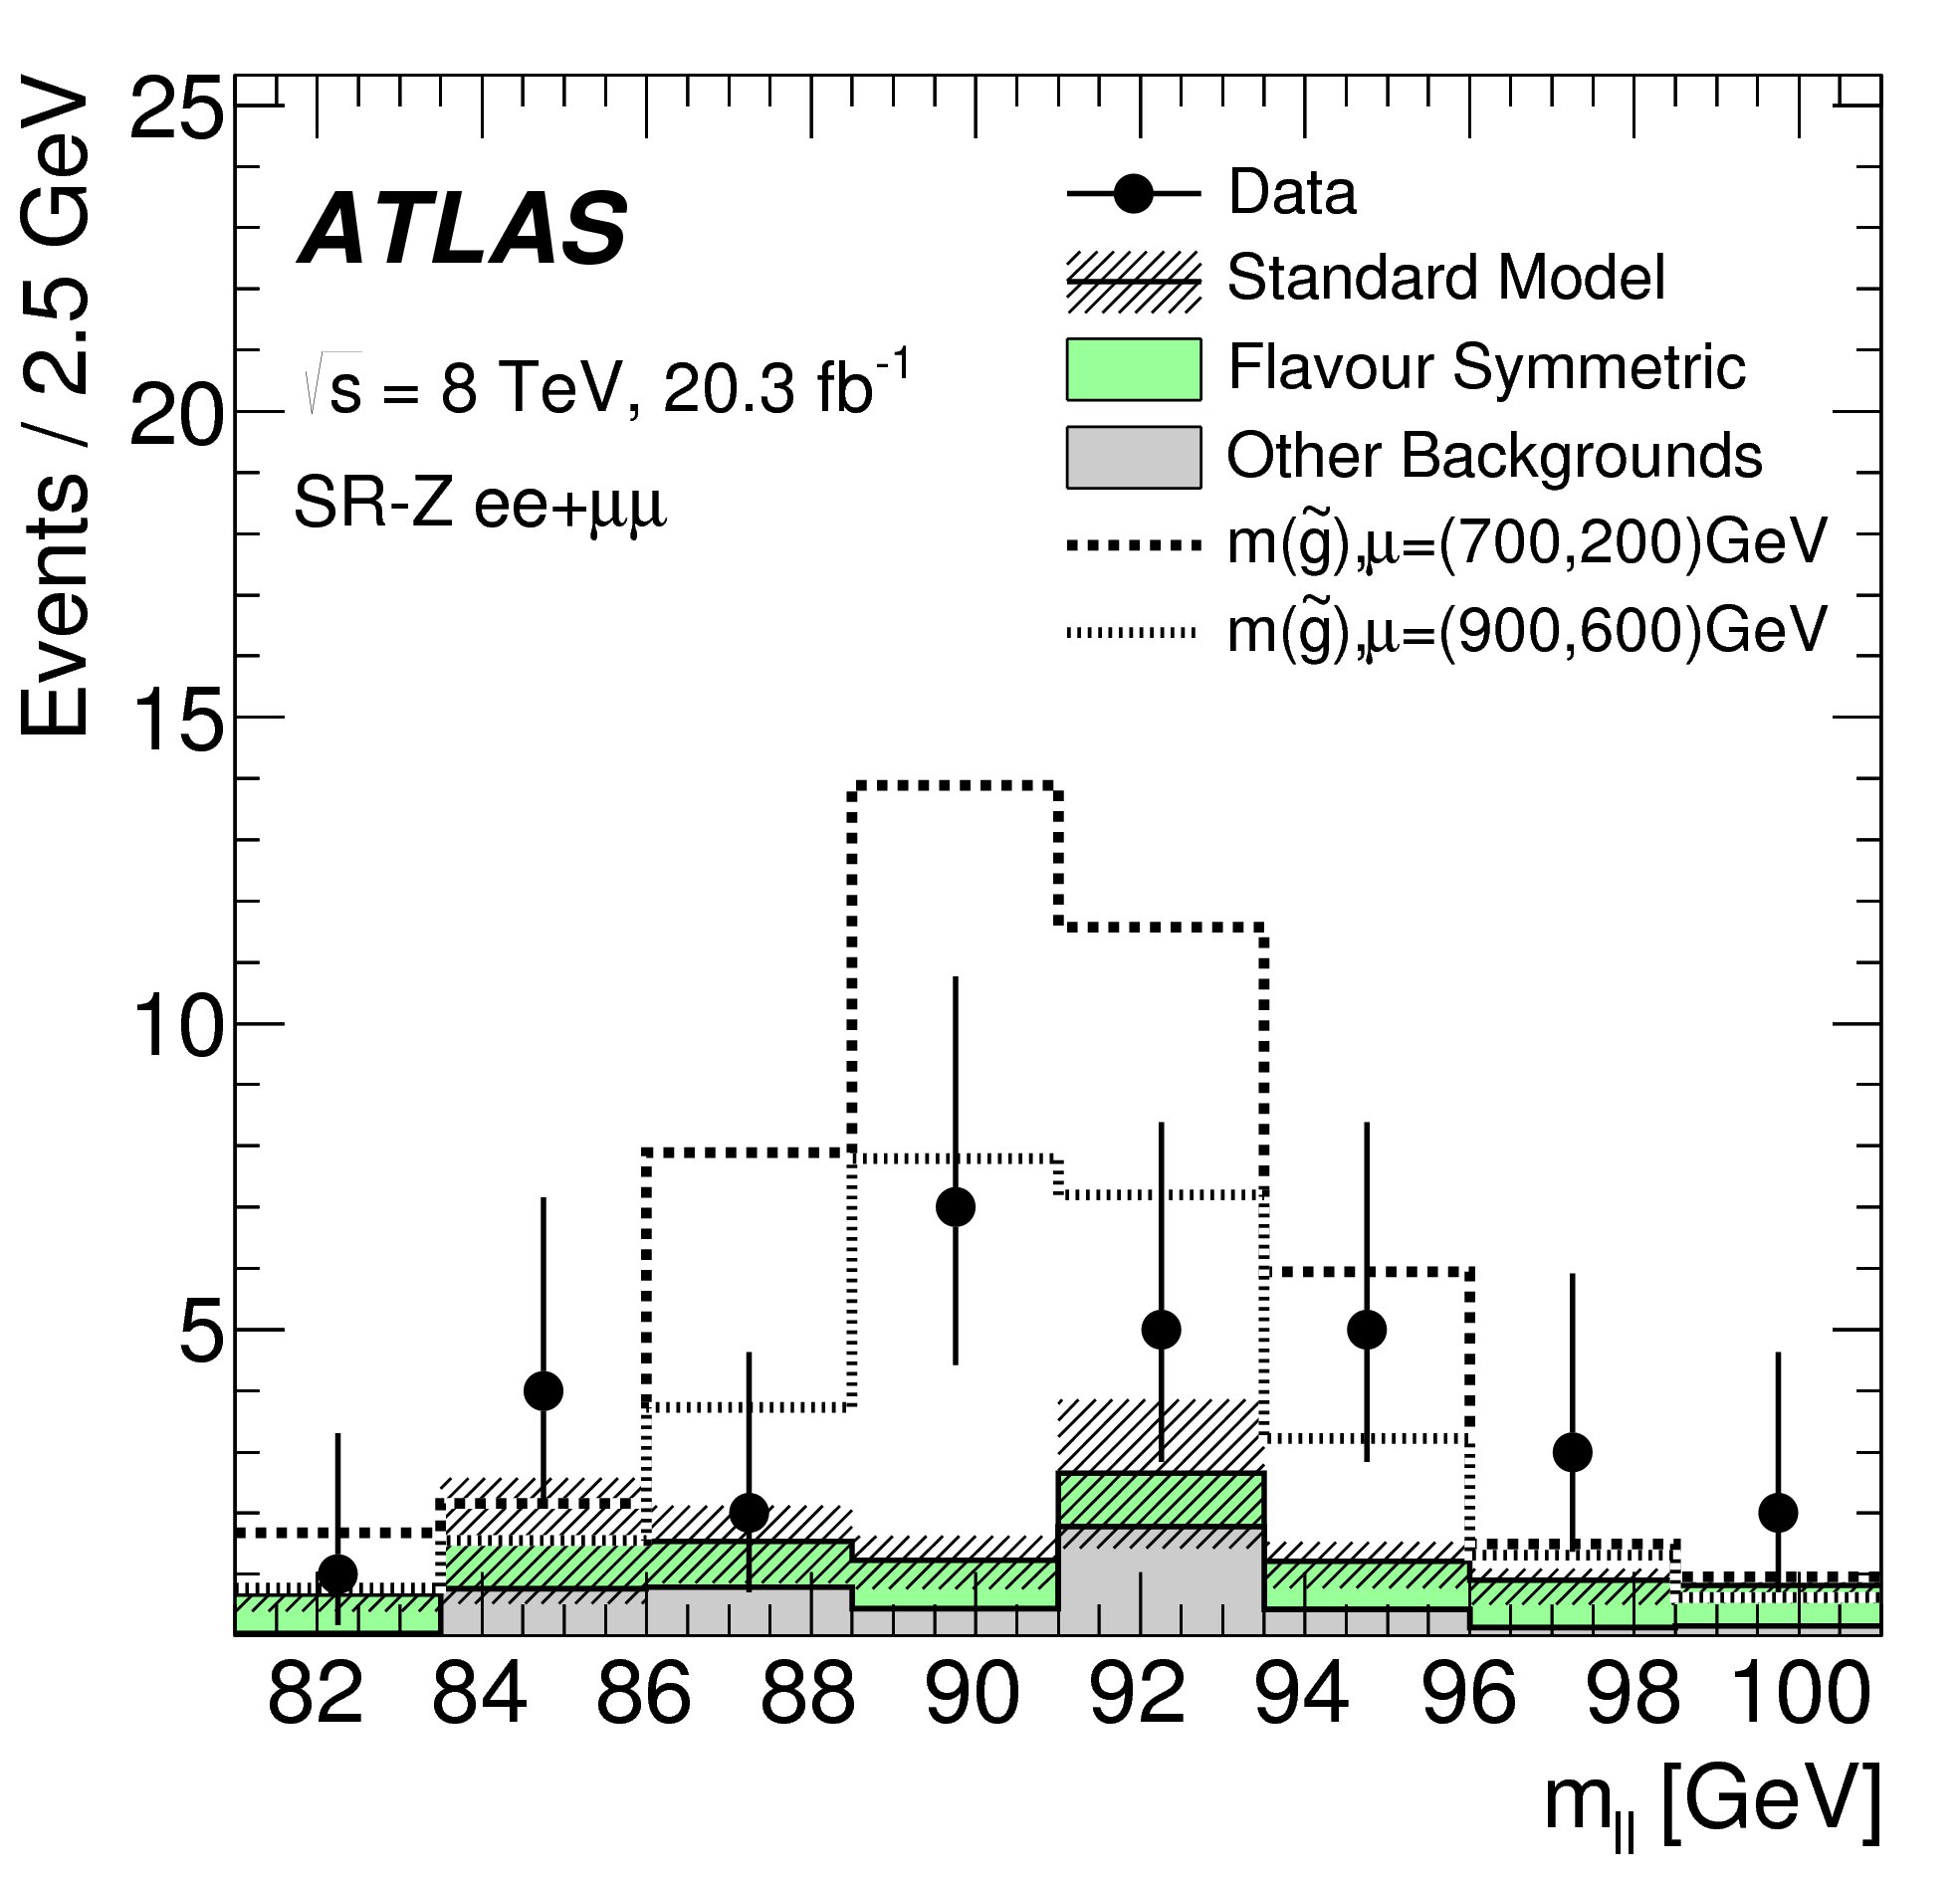
\includegraphics[width=.9\linewidth]{figures/theory/figaux_12a.png}
\caption{ Results of an 8 \tev~search performed by the ATLAS collaboration in a signal region targeting events like those in \autoref{fig:simpodel}. The \ac{SM} backgrounds are shown with their full uncertainties based on data-driven background estimations, and two signals are superimposed on the distribution. The observed datapoints are higher than the expected background, with a total excess of 3.0$\sigma$. The events in the signal region are displayed as a function of \mll, the invariant mass of the event's leading leptons \cite{SUSY-2014-10}.}
\label{fig:atlas_8tev}
\end{figure}
\end{centering}

Both searches also identified events with two leptons that weren't consistent with an on-shell $Z$ decay, and in this region, an excess with a local significance of 2.4$\sigma$ was observed by \ac{CMS}, shown in \autoref{fig:cms_8tev}. No excess was observed by the ATLAS collaboration in a signal region with identical kinematic cuts \cite{SUSY-2014-10}. 

\begin{centering}
\begin{figure}[!hbt]
\myfloatalign
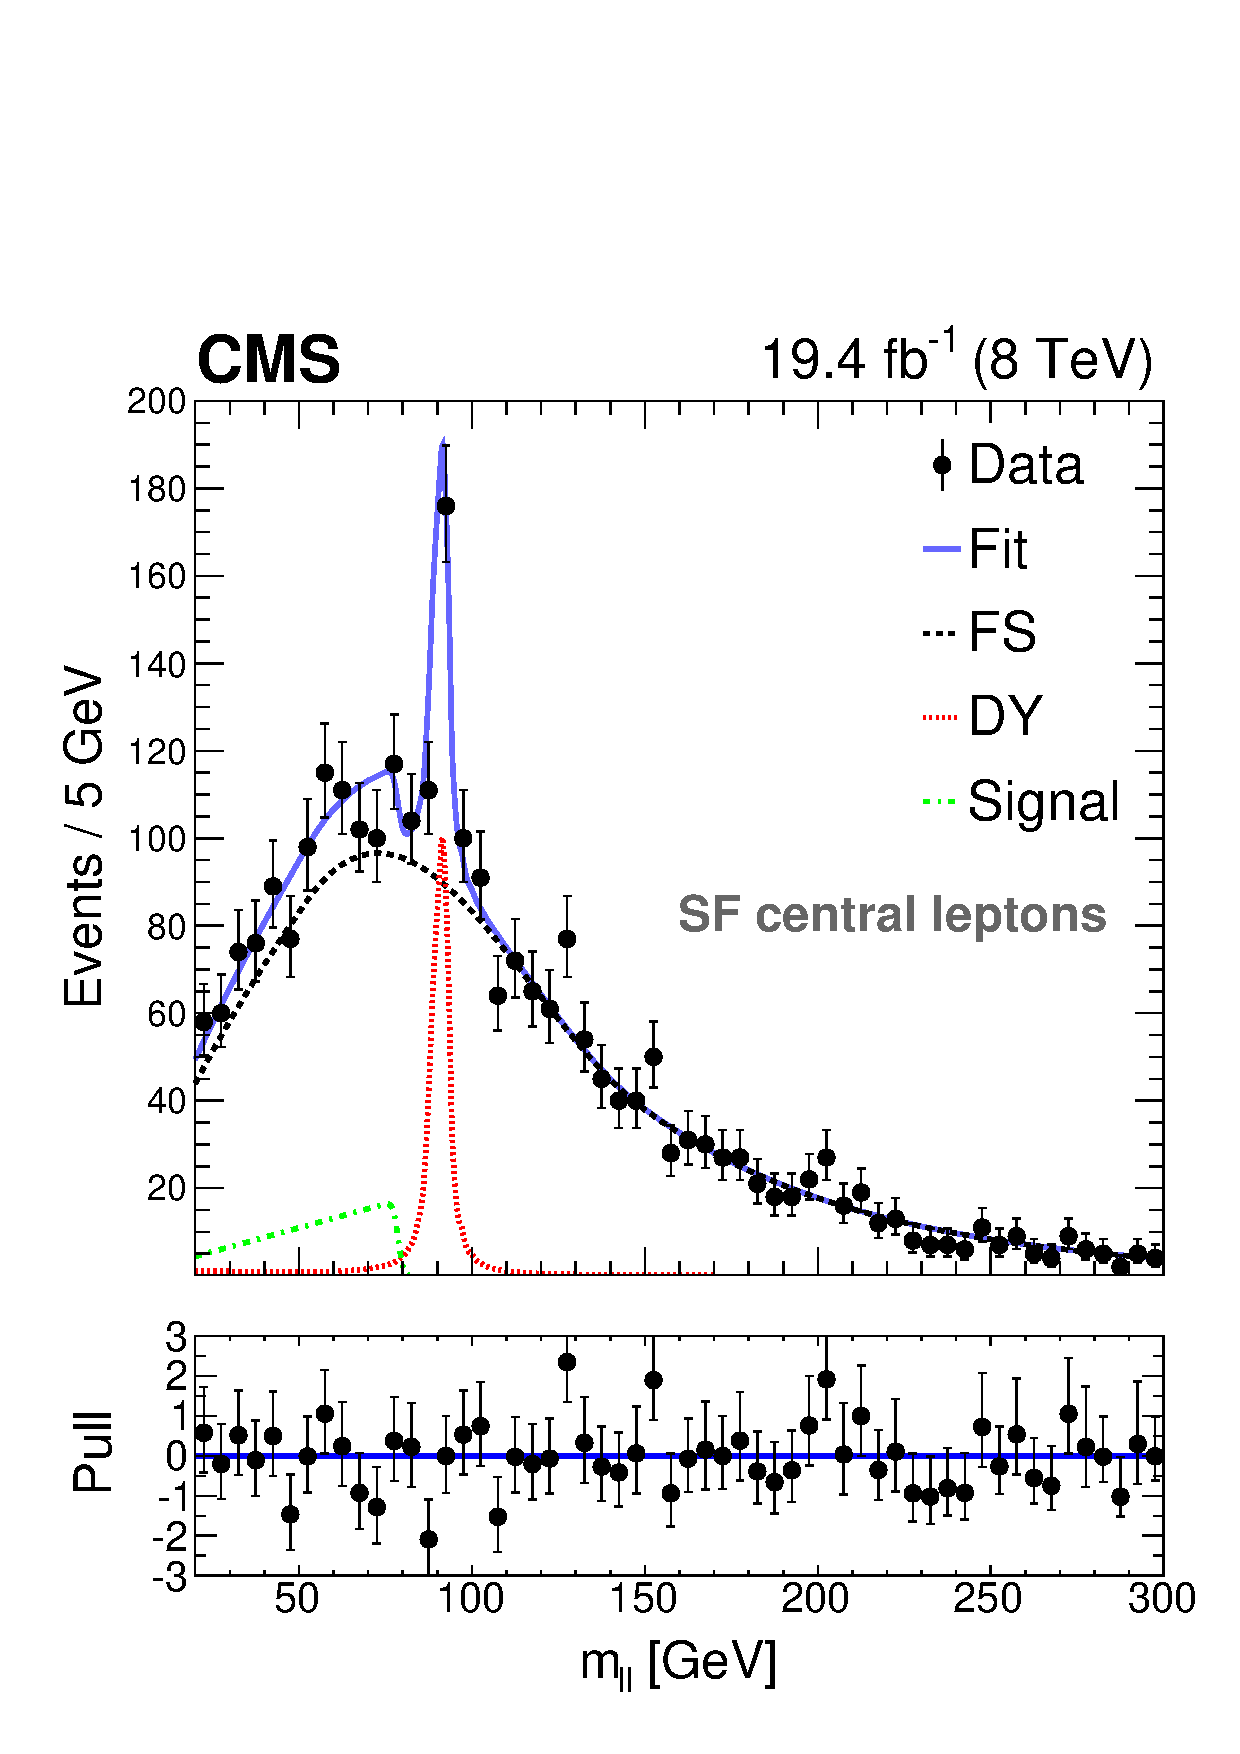
\includegraphics[width=.9\linewidth]{figures/theory/H1_FIT_SF_CE.pdf}
\caption{ Results of an 8 \tev~search performed by the \ac{CMS} collaboration in a signal region including a broad range of \mll. A 2.4$\sigma$ local excess is seen in the low \mll~region, and no excess of events is seen in the region with \mll~consistent with an on-shell $Z$ boson. The data is fit based on a data driven estimate of the flavor symmetric background (FS) and the Drell-Yan background (DY), with an additional component for the signal \cite{CMS2}.}
\label{fig:cms_8tev}
\end{figure}
\end{centering}

These two excesses generated significant interest in the two lepton channel, and both \ac{CMS} and ATLAS produced preliminary results in December 2015 with the first 3.2 fb$^{-1}$ of 13 \tev~data. ATLAS again reported an excess on the $Z$ mass peak \cite{ATLAS-CONF-2015-082}, shown in \autoref{fig:atlas_eoye}, while \ac{CMS} saw no excesses \cite{CMS-PAS-SUS-15-011}. 

\begin{centering}
\begin{figure}[!hbt]
\myfloatalign
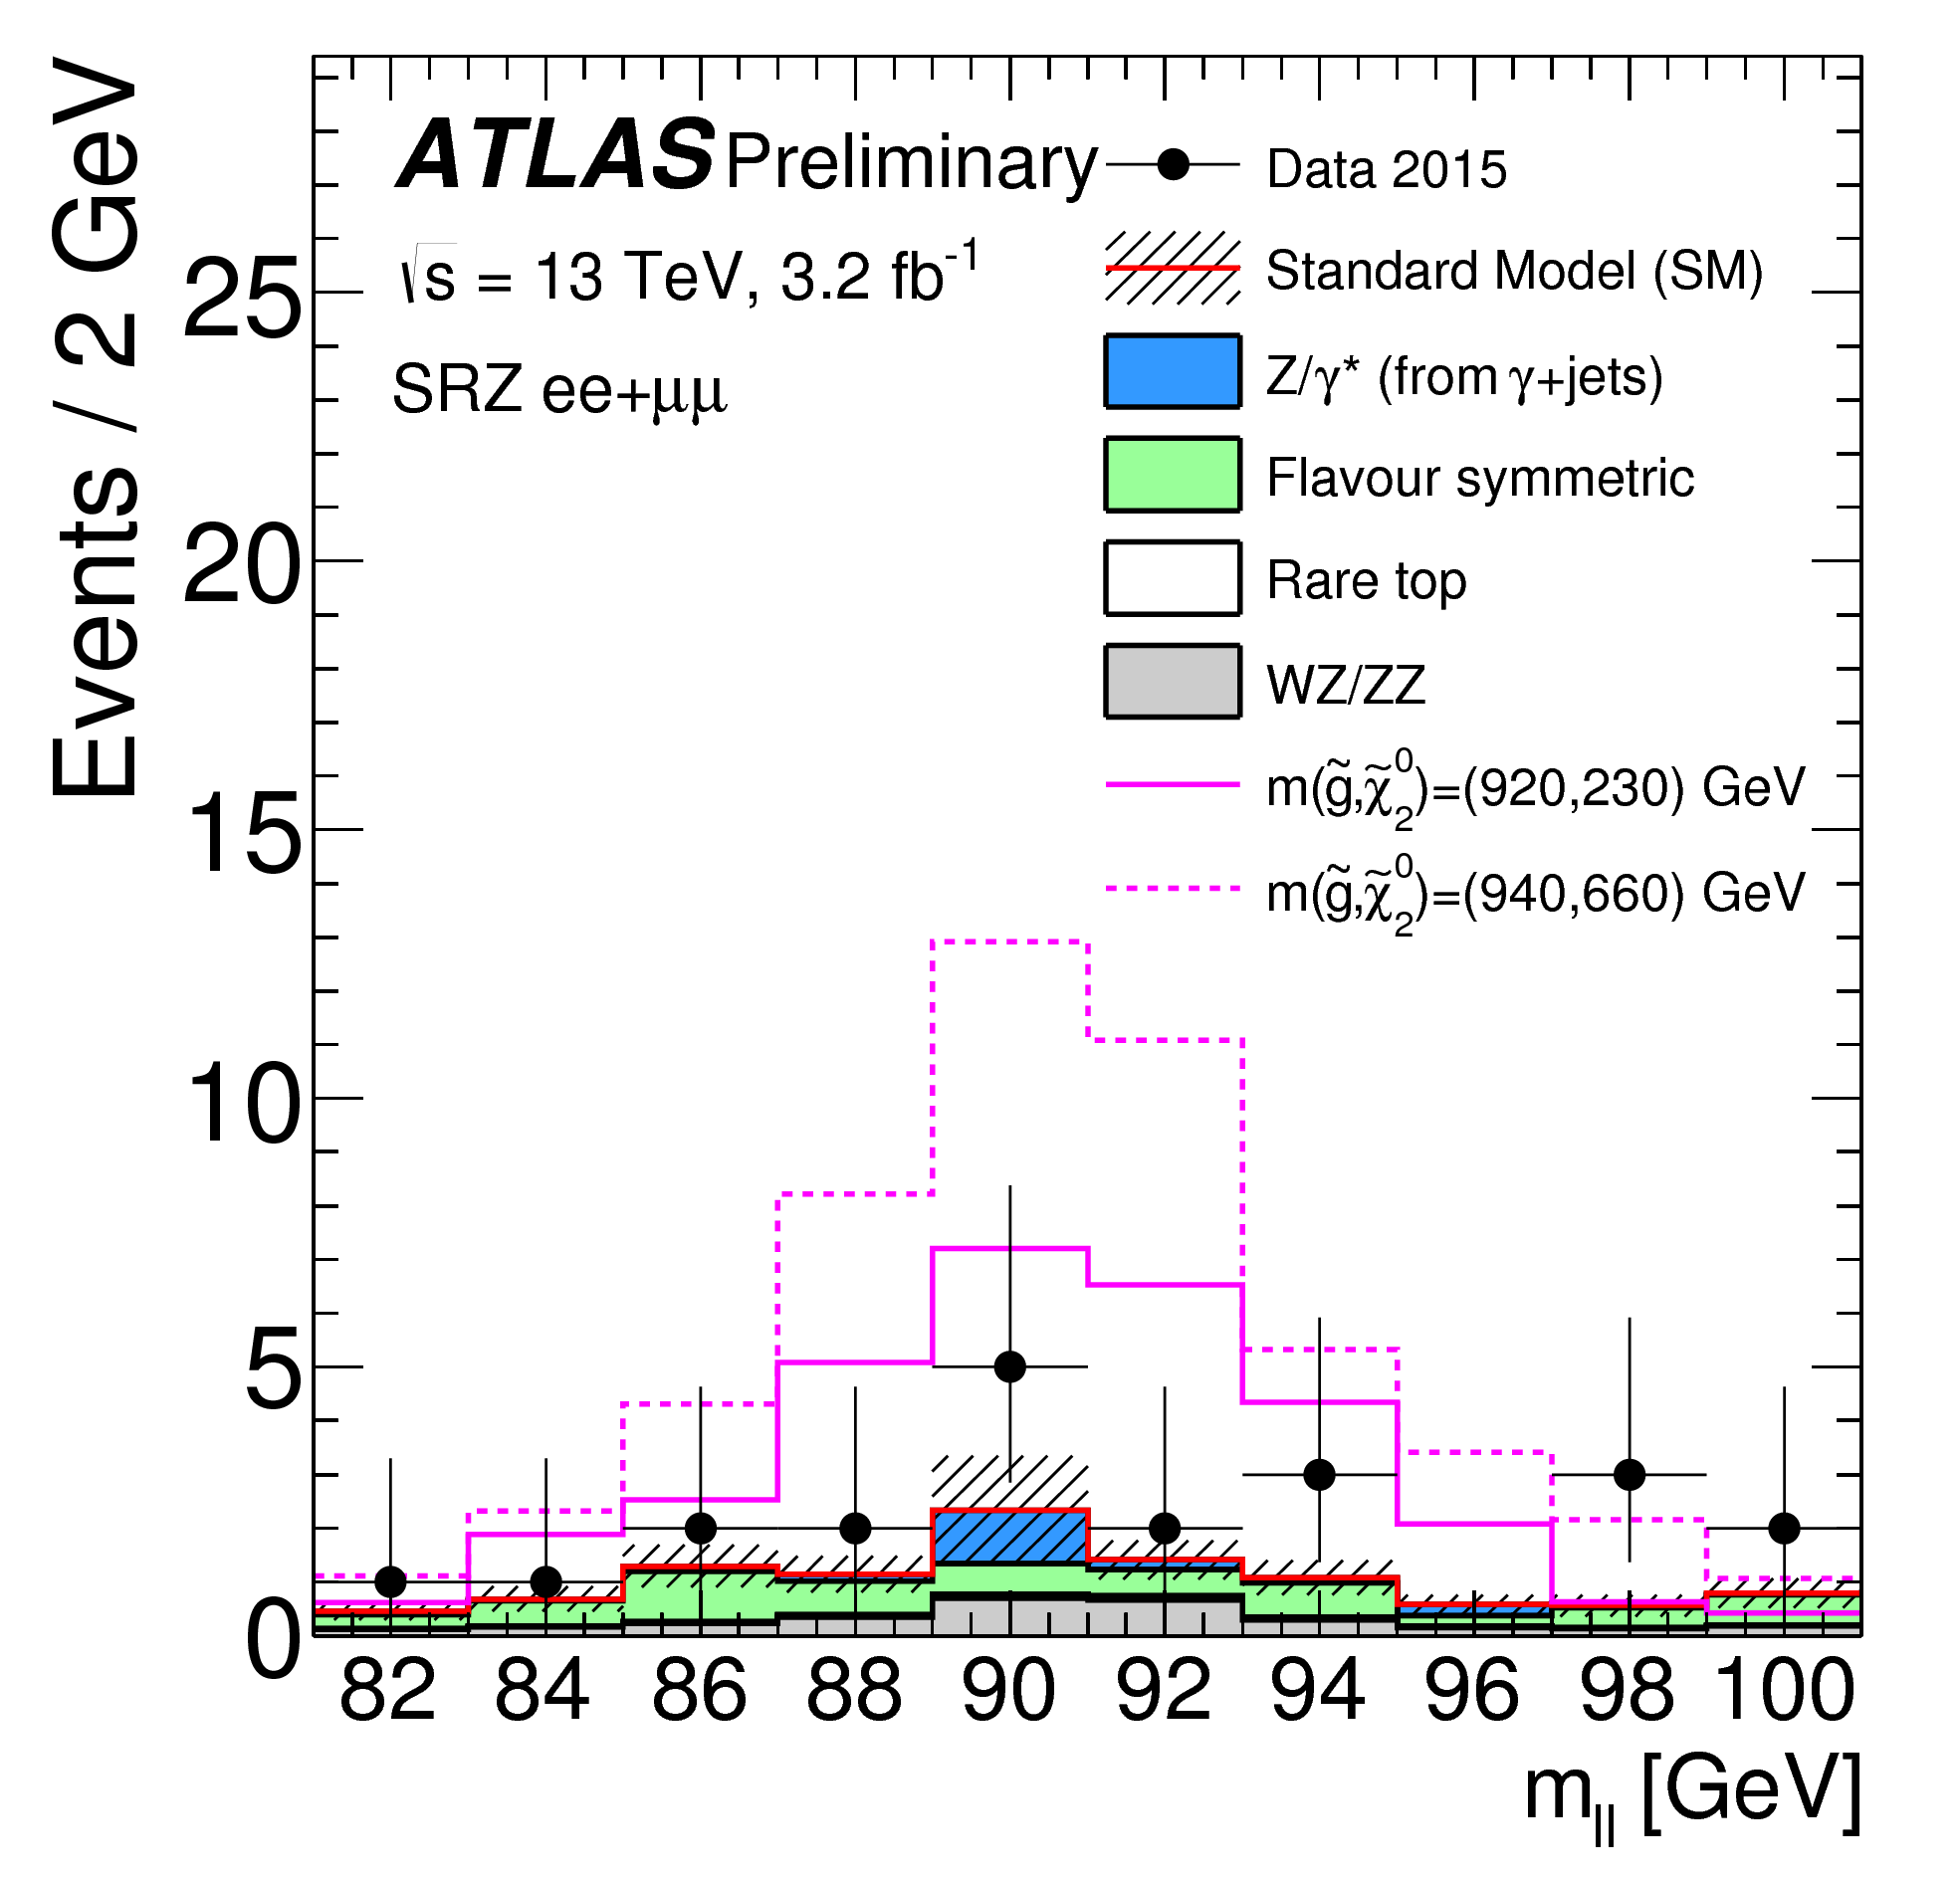
\includegraphics[width=.9\linewidth]{figures/theory/fig_05.png}
\caption{ Preliminary results from a 13 \tev~search targeting the same signal region as \autoref{fig:atlas_8tev}, performed on 3.2 fb$^{-1}$ of 2015 data. Flavor symmetric and \dyjets backgrounds are taken from data-driven methods, while the other backgrounds are taken from \ac{MC}. They are compared to the data, which shows a 2.2$\sigma$ excess of events. Distributions from two signal points are superimposed \cite{ATLAS-CONF-2015-082}.}
\label{fig:atlas_eoye}
\end{figure}
\end{centering}

Aside from the history of excesses, the channel is well-motivated from a theoretical perspective. The pair production of gluinos is the most common production mode for most \ac{SUSY} models which describe gluinos with much smaller masses than squarks. \autoref{fig:gluino_xs} shows the production cross-sections for sparticles at the \ac{LHC} as a function of their mass. The specific decay considered in these simplified models does not have the largest branching ratio of all possible decays; even considering only changes to the \ac{SM} decays involved, a $Z\rightarrow qq$ decay is roughly seven times more likely than $Z\rightarrow\ell\ell$. However, processes with higher branching ratios, like those producing an all-jet final state, often have much higher \ac{SM} backgrounds, making them difficult to identify, even if they occur more frequently. This final state balances \ac{SM} backgrounds and branching ratios, and when compared to other searches performed by the ATLAS collaboration, has competitive sensitivity to \ac{SUSY}. 

\begin{centering}
\begin{figure}[!hbt]
\myfloatalign
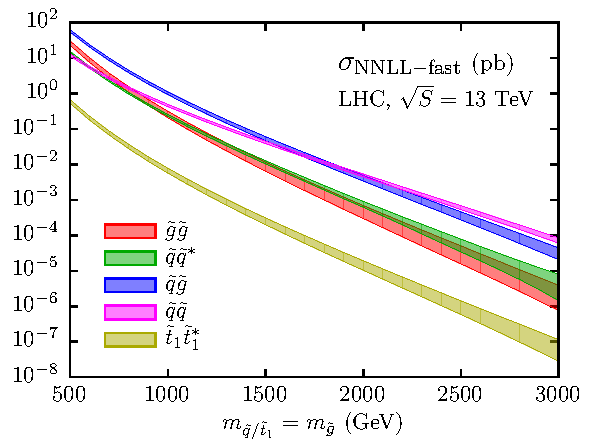
\includegraphics[width=.9\linewidth]{figures/theory/nnllfast_wpresc_total.pdf}
\caption{ 13 \tev~production cross-sections for sparticles, as a function of sparticle mass \cite{1607.07741}.}
\label{fig:gluino_xs}
\end{figure}
\end{centering}


\section{Monte Carlo Generation}
\label{sec:MC_gen}

The complex events of the \ac{LHC} are difficult to model, but modeling them is crucial to analyzers' understanding of \ac{SM} backgrounds and potential signals. To simplify the modeling process, particle interactions are broken down into very small steps, each with associated probabilities of various outcomes. This modeling method is called \acf{MC}, and, at the \ac{LHC} it is broken into several larger steps which are each handled by different software. 

The first step, discussed in \autoref{sec:pp_collisions}, is to determine the energies of the initial particles in a collision, which are provided by several different \ac{PDF} sets. These distributions come from experimental measurements, though there is some variation between different sets. Three different sets are used in this analysis: NNPDF2.3LO \cite{Ball:2012cx} and NLO CT10 \cite{Lai:2010vv} for background and signal processes, and MSTW 2008 \cite{0901.0002} for pile-up events, discussed more in \autoref{sec:pileup}. 

With the initial states of the constituents of the protons described by these probabilistic models, the next step is to model the hard scattering process resulting from the interaction of two of these particles. This is accomplished by a generator, which calculates the cross-sections of the Feynman diagrams of a given process. In particular, these generators typically produce \textit{matrix elements}, which describe the probability to go from an initial to final state via a hard scattering, including the kinematics of the output. The generator uses these matrix elements to assign one of these hard scattering final states to each event. These hard scattering outputs are then passed to the next step, where parton showering, fragmentation, final and initial state radiation, and hadronization can occur.

The calculation of these diagrams can become very complicated when more and more loops are allowed. The simplest calculations, which include diagrams without any loops, are referred to as \ac{LO}, while calculations including diagrams with one loop are called \ac{NLO}, and additional Ns can be added to describe more complex calculations. In addition, the total cross-section for a given process can be calculated at a higher order and used to scale the overall number of events generated for the process. 

These calculations can also be tuned, varying parameters in the generation to create outputs that most closely match experimental data. In some cases, this can mean that a tune might include values for certain physical quantities that are different from their measured values because this configuration ultimately produces a result more similar to data. 

Examples of generators include {\sc MadGraph5\_aMC@NLO} \cite{Alwall:2014hca}, {\sc Powheg Box} \cite{PowhegBOX1,PowhegBOX2,PowhegBOX3}, and \sherpa~\cite{sherpa}. Each has different strengths and is used to describe processes that best match those strengths. {\sc Powheg Box}, for example, cannot perform its own parton showering, and must be interfaced with another generator, typically {\sc Pythia} \cite{Sjostrand:2006za}, in order to describe any physics processes beyond the hard scattering, which can cause discontinuities in its predictions for large numbers of partons. However, it can calculate matrix elements at \ac{NLO}, giving it an advantage in calculating some complex processes. \sherpa performs its own parton showering, but in most cases calculates its matrix elements at \ac{LO}. The main advantage {\sc MadGraph5\_aMC@NLO}, which must also be interfaced with another generator perform parton showering, is its simple user interface. This makes it popular for producing \ac{SUSY} signal samples, which must be done by each analysis team searching for a different \ac{SUSY} process. 

Once the final state particles of the hard interaction and showering have been calculated, the pile-up of the \ac{LHC} (described in \autoref{sec:pileup}) must be accounted for. Events called \textit{minimum bias} are generated to match the overall production of the \ac{LHC} collisions, with no preselection. These events are overlaid on the original hard scatter to produce a more realistic representation of the many simultaneous interactions observed in the ATLAS detector.

This collection of particles must then be translated into signals in the detector. Their trajectories in the magnetic fields of the detector, their interactions in each layer, and the way these interactions deposit charge in each subdetector are modeled in software called {\sc GEANT4}~\cite{Agostinelli:2002hh}. In this software, every piece of the ATLAS detector is modeled, including the magnetic field and the many different materials. Particles then follow trajectories through the simulated detector and interact with the different materials based on several preprogrammed options for each material. For example a photon traveling through a material could continue along its trajectory, convert into a positron-electron pair, or deposit energy. As it crosses into a new material, a new set of options opens up for interactions. The particle is tracked until all of its energy is lost or it exits the geometry of the simulation.

The model of the detector used for this process is iteratively perfected by comparing data to \ac{MC}. \autoref{fig:geant} shows an example of a discrepancy between the simulation and observed data in the number of secondary vertices in a pixel module, which should correspond to the amount of material in the area. Observations of discrepancies like this can be used to correct the materials in the simulation. 

\begin{centering}
\begin{figure}[!hbt]
\myfloatalign
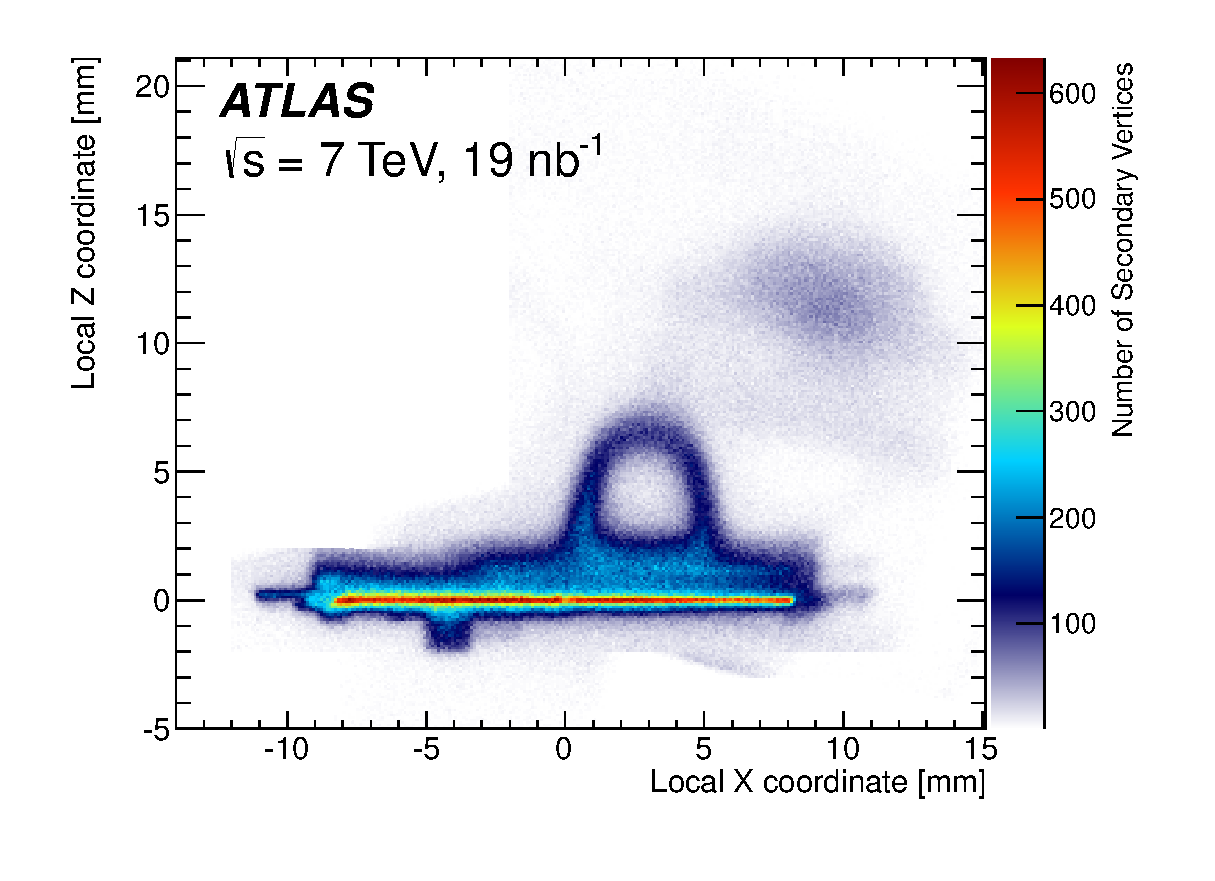
\includegraphics[width=.9\linewidth]{figures/theory/fig_10a.eps}
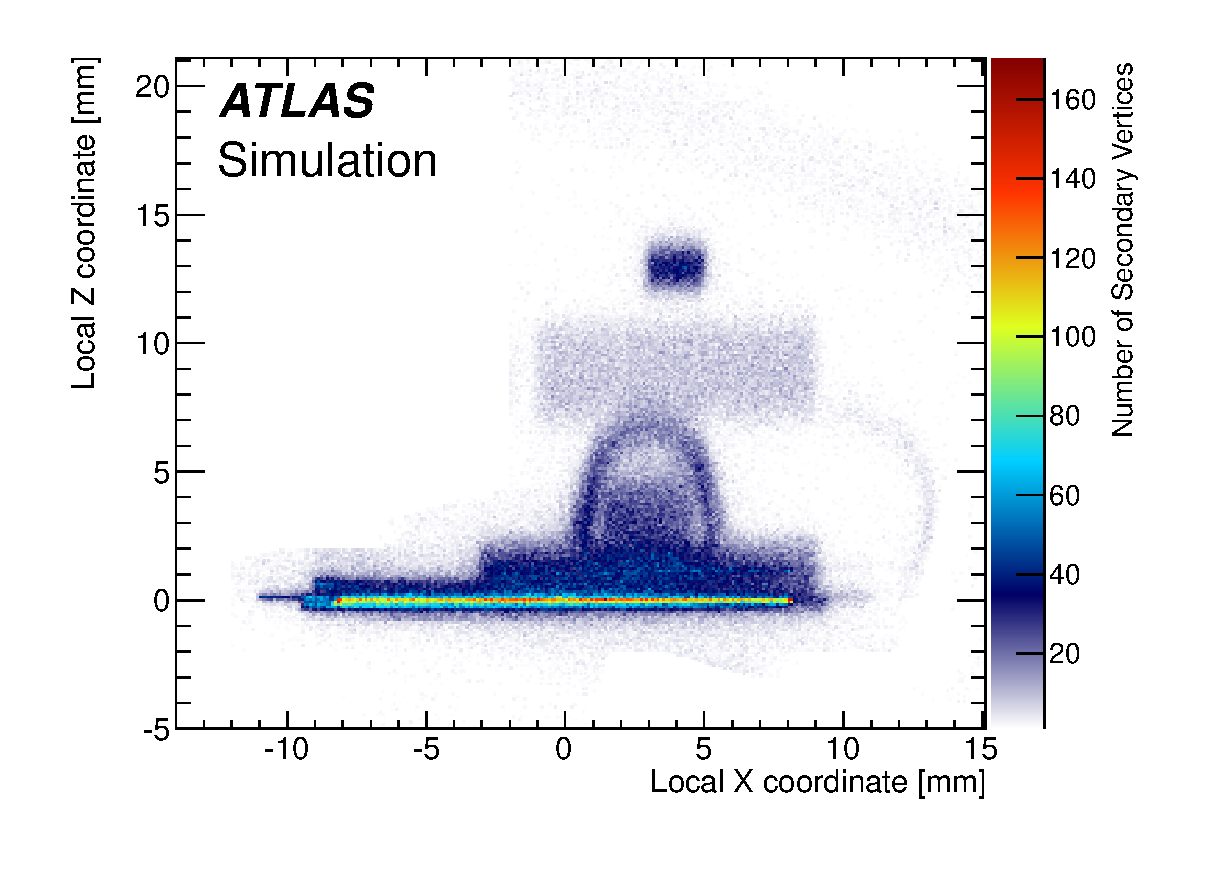
\includegraphics[width=.9\linewidth]{figures/theory/fig_10b.eps}
\caption{Number of secondary vertices in a module in the first layer of the pixel detector in data (top) and \ac{MC} (bottom). There are more events in the data than the \ac{MC} \cite{PERF-2015-06}.}
\label{fig:geant}
\end{figure}
\end{centering}

Custom ATLAS code converts the energy deposited in active sensors into signals that resemble the expected detector response. These responses are typically very complicated with many parameters, and are frequently iterated on to best match the data. Electronic noise must also be added to correctly approximate the operating conditions of the detector. Additional alterations to this signal translation, including dead sensors and misalignments of the detector, can also be added at this stage. 

Once the simulated particles have been converted into detector signals, the same reconstruction software used on data can be used on the \ac{MC}, converting the detector signals back into particle interpretations. This reconstruction process is described in \autoref{ch:reconstruction}. The original information about the particles from the generator, referred to as \textit{truth} information, is also kept, and can be compared to the reconstruction output to study its efficacy.






